\chapter{Casos de estudo}
\label{cap:avaliacao}

Os dois capítulos anteriores descreveram os métodos escolhidos e o sistema que os põe a funcionar.
Este determina o que cada um deles vale. Descreve-se primeiro o desenho experimental e as métricas
utilizadas. Seguem-se quatro casos de estudo: três correspondem às questões de investigação, e o
quarto ao comportamento do sistema em operação, onde as escolhas dos capítulos anteriores encontram
dados que não estavam disponíveis quando foram tomadas.

\section{Desenho experimental e métricas}
\label{sec:av_desenho}

Esta secção fixa a forma comum a todos os casos de estudo e define as medidas empregues, com
especial atenção ao valor que cada uma assume na ausência de informação.

Cada caso de estudo segue quatro passos, representados na Figura~\ref{fig:av_forma}: a pergunta, o
procedimento de medição e a alternativa contra a qual a comparação é feita, o resultado obtido, e o
que esse resultado não permite concluir. O quarto passo é o que distingue uma avaliação de uma
demonstração. Os valores medidos sobre conjuntos históricos congelados são produzidos por procedimentos
automáticos com semente fixa e reproduzem-se exatamente. Duas classes de valor não têm essa propriedade, e são identificadas onde aparecem. Os valores
lidos do sistema em operação são instantâneos datados, que crescem com o canal. Os que dependem de
cotações reajustadas pela fonte podem variar na terceira casa decimal.

\begin{figure}[ht]
\centering
\begin{tikzpicture}[font=\small, >={Stealth[length=2.2mm]},
  et/.style={draw, rounded corners=2pt, align=center, text width=2.5cm, minimum height=1.15cm,
             inner sep=3pt, fill=black!4},
  ult/.style={et, fill=black!14, draw=black!60, thick},
  err/.style={draw, rounded corners=2pt, align=center, text width=3.6cm, minimum height=0.95cm,
              inner sep=3pt, fill=white},
]
  \node[et] (a) {\textbf{1.} a pergunta};
  \node[et, right=5mm of a] (b) {\textbf{2.} como se mede, e contra quê};
  \node[et, right=5mm of b] (c) {\textbf{3.} o resultado};
  \node[ult, right=5mm of c] (d) {\textbf{4.} o que não se conclui};
  \foreach \xa/\xb in {a/b, b/c, c/d} \draw[->, thick, black!55] (\xa) -- (\xb);

  \node[err, below=9mm of b] (fp)
    {\footnotesize \textbf{falso positivo}\\[-1pt]\footnotesize gasta a atenção de quem lê};
  \node[err, below=9mm of c] (fn)
    {\footnotesize \textbf{falso negativo}\\[-1pt]\footnotesize deixa passar o dia que importava};
  \node[font=\scriptsize, text=black!60, align=center] at ($(fp)!0.5!(fn) + (0,-1.05)$)
    {os dois erros custam coisas diferentes, e nenhuma medida deste capítulo os trata como iguais};
\end{tikzpicture}
\caption[A forma comum aos quatro casos de estudo]{A forma seguida por todos os casos de estudo. O
quarto passo delimita o alcance de cada resultado. Em baixo, os dois tipos de erro que as medidas
desta secção equilibram, e o custo distinto de cada um no domínio de aplicação.}
\label{fig:av_forma}
\end{figure}

Todas as medidas assentam nas quatro combinações entre o que o sistema afirma e o que se verifica.
A precisão é a fração de acertos entre as ocasiões em que o sistema falou,
$\mathrm{VP}/(\mathrm{VP}+\mathrm{FP})$; a cobertura, também chamada \emph{recall}, é a fração dos
casos relevantes que foram assinalados, $\mathrm{VP}/(\mathrm{VP}+\mathrm{FN})$. As duas variam em
sentidos opostos, e uma regra que assinale quase tudo atinge cobertura elevada com precisão baixa.

O $F_1$ é a média harmónica das duas, $2PC/(P+C)$, e aproxima-se do pior dos dois valores, o que
impede que um extremo seja premiado. Para o \emph{z}-score, com precisão $0{,}381$ e cobertura
$0{,}800$, resulta $0{,}516$; para a regra de limiar fixo, com precisão $0{,}122$ e cobertura
$0{,}992$, resulta $0{,}218$.

A precisão@$k$ aplica-se à recuperação, que devolve uma lista ordenada de que o utilizador lê apenas
o início. Mede a fração dos $k$ primeiros resultados que são relevantes \autocite{manning2008ir},
com $k = 5$, valor que corresponde ao que cabe num alerta.

A \gls{PRAUC} aplica-se à triagem, que devolve uma probabilidade e não uma decisão. Cada limiar
possível produz um par de precisão e cobertura, e o conjunto desses pares desenha a curva de
precisão e cobertura; a área sob essa curva resume o modelo em todos os limiares simultaneamente,
em vez de o julgar num limiar escolhido manualmente. É preferível à percentagem de acertos porque,
com classes desequilibradas, responder invariavelmente que a notícia não é material acerta
$62{,}2\%$ das vezes sem qualquer aprendizagem.

O índice de Brier observa o valor da probabilidade e não a ordenação, sendo a média do quadrado do
erro entre a probabilidade anunciada e o resultado observado, com valores menores a corresponder a
melhor desempenho. O quadrado penaliza de forma mais do que proporcional os enganos confiantes, que
é a propriedade adequada num sistema que exibe percentagens a um destinatário sem meios para as
questionar.

Uma medida lida sem o valor que lhe corresponde na ausência de informação conduz à conclusão errada,
e este capítulo documenta três ocasiões em que isso sucedeu. A Tabela~\ref{tab:av_metricas} fixa
esse valor para cada medida.

\begin{table}[!htbp]
\caption[As medidas utilizadas e o valor que cada uma tem sem informação]{Cada medida, a pergunta a
que responde, o valor que um método sem informação obtém, e o caso de estudo em que é utilizada. A
coluna central é a que impede a leitura otimista de uma percentagem isolada.}
\label{tab:av_metricas}
\centering
\small
\begin{tabular}{L{0.17\textwidth} L{0.33\textwidth} L{0.24\textwidth} C{0.11\textwidth}}
\toprule
\tabhead{Medida} & \tabhead{Responde a} & \tabhead{Valor sem informação} & \tabhead{Utilizada em} \\
\midrule
Amplitude de disparo & O detetor comporta-se do mesmo modo em empresas distintas? &
zero é o ótimo, e é atingível sem informação & \gls{QI}1 \\
\addlinespace
$F_1$ & Acerta quando fala, e fala quando devia? & depende dos dados & \gls{QI}1 \\
\addlinespace
Precisão@5 & Das cinco apresentadas, quantas são relevantes? & $0{,}240$, medido por escolha
aleatória & \gls{QI}2 \\
\addlinespace
\gls{PRAUC} & Ordena bem, qualquer que seja o limiar? & $0{,}378$, a prevalência do bloco de teste &
\gls{QI}3 \\
\addlinespace
Índice de Brier & A percentagem anunciada corresponde à frequência observada? & $0{,}622$, obtido
por anunciar sempre a unidade & \gls{QI}3 \\
\bottomrule
\end{tabular}
\end{table}

A primeira linha da Tabela~\ref{tab:av_metricas} é a única medida do capítulo que não utiliza
rótulos. A amplitude de disparo é a diferença entre a taxa a que o detetor assinala na empresa em que mais
fala e a taxa na empresa em que menos fala. Assenta num único princípio: um detetor universal deve
comportar-se de forma semelhante em empresas distintas. A sua propriedade menos
evidente, e que a Secção~\ref{sec:av_qi1} desenvolve, é a de que o ótimo é atingível sem qualquer
informação.

\section{Deteção consistente entre empresas}
\label{sec:av_qi1}

O primeiro caso de estudo responde à \gls{QI}1: um \emph{z}-score deslizante deteta movimentos
invulgares de forma mais consistente entre empresas do que uma regra de limiar fixo. A resposta é
afirmativa, com uma margem de mais de vinte vezes na medida principal.

\subsection{Procedimento}

A avaliação utiliza três anos de cotações diárias de quinze empresas de grande capitalização, entre
junho de 2023 e junho de 2026, o que corresponde a aproximadamente setecentos e cinquenta dias por
empresa. O conjunto é distinto da lista de doze empresas monitorizadas em produção, pela razão
enunciada na Secção~\ref{sec:met_dados}: a avaliação exige variedade de volatilidade, e a lista
implantada é uma decisão de produto.

O argumento principal não recorre a rótulos. Um detetor destinado a assinalar dias raros deve
disparar a uma taxa semelhante em empresas distintas; se dispara com frequência elevada numa e
raramente noutra, o que está a medir é a volatilidade da empresa e não a raridade do dia. Como
argumento de apoio utiliza-se um rótulo aproximado, que classifica como extremo um dia situado no
percentil noventa e nove dos retornos da própria empresa. O rótulo é imperfeito, por ser ele próprio
relativo à volatilidade, e ocupa por isso a posição secundária.

\subsection{Resultado}

A Figura~\ref{fig:av_amplitude} resume as duas medidas, e a primeira delas é a que sustenta a
conclusão desta secção: o que distingue os dois métodos não é o nível a que disparam, mas o facto de
o limiar fixo acompanhar a volatilidade de cada ação enquanto o \emph{z}-score se mantém quase
constante entre elas.


\begin{figure}[ht]
\centering
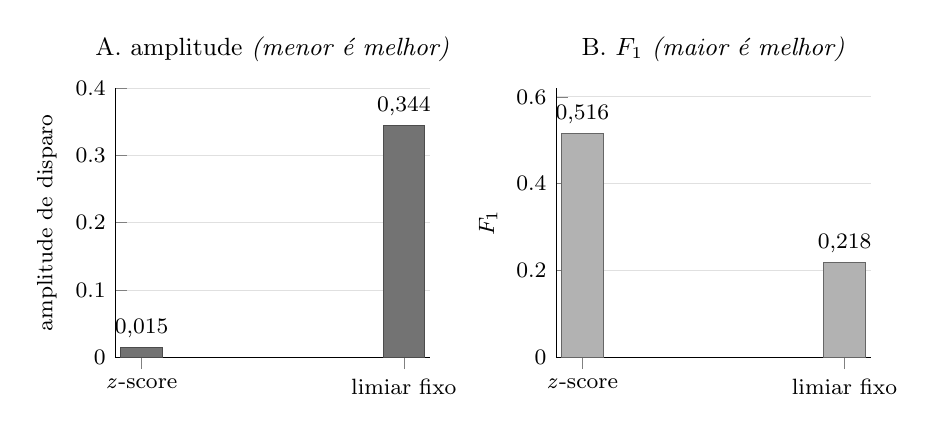
\begin{tikzpicture}
\begin{axis}[
  name=esq, width=0.46\textwidth, height=5.0cm, ybar, bar width=15pt,
  ymin=0, ymax=0.40, symbolic x coords={zscore, fixo}, xtick=data,
  xticklabels={\emph{z}-score, limiar fixo}, ylabel={amplitude de disparo},
  nodes near coords, point meta=explicit symbolic,
  every node near coord/.append style={font=\footnotesize},
  title={\small A. amplitude \emph{(menor é melhor)}},
  tick label style={font=\footnotesize}, label style={font=\footnotesize},
  ymajorgrids, grid style={black!12}, axis lines*=left,
]
\addplot[fill=black!55, draw=black!70] coordinates {(zscore,0.015) [0,015] (fixo,0.344) [0,344]};
\end{axis}
\begin{axis}[
  name=dir, at={(esq.right of origin)}, anchor=left of origin, xshift=1.6cm,
  width=0.46\textwidth, height=5.0cm, ybar, bar width=15pt,
  ymin=0, ymax=0.62, symbolic x coords={zscore, fixo}, xtick=data,
  xticklabels={\emph{z}-score, limiar fixo}, ylabel={$F_1$},
  nodes near coords, point meta=explicit symbolic,
  every node near coord/.append style={font=\footnotesize},
  title={\small B. $F_1$ \emph{(maior é melhor)}},
  tick label style={font=\footnotesize}, label style={font=\footnotesize},
  ymajorgrids, grid style={black!12}, axis lines*=left,
]
\addplot[fill=black!30, draw=black!60] coordinates {(zscore,0.516) [0,516] (fixo,0.218) [0,218]};
\end{axis}
\end{tikzpicture}
\caption[As duas medidas da primeira questão]{As duas medidas, lado a lado. Em A, a diferença entre
a taxa máxima e a taxa mínima entre as quinze empresas; o limiar fixo assinala $0{,}9\%$ dos dias na
empresa mais calma e $35{,}3\%$ na mais volátil, enquanto o \emph{z}-score se mantém entre $1{,}6\%$
e $3{,}1\%$ em todas. Em B, o desempenho contra o rótulo aproximado.}
\label{fig:av_amplitude}
\end{figure}

A amplitude da taxa de disparo é de $0{,}015$ para o \emph{z}-score e de $0{,}344$ para o limiar
fixo, uma diferença superior a vinte vezes. Contra o rótulo aproximado, o \emph{z}-score obtém
$F_1 = 0{,}516$ e o limiar fixo $0{,}218$.

A comparação envolve uma assimetria de tratamento. A janela do \emph{z}-score é variada mais adiante
nesta secção, ao passo que o limiar de três por cento da regra fixa é o valor convencional e não foi
otimizado. O que a comparação estabelece com segurança não é que nenhum limiar fixo obteria melhor
resultado, mas que um limiar fixo mede uma quantidade diferente da pretendida, porque a mesma
percentagem corresponde a raridades distintas em empresas distintas. Este argumento não depende do
valor escolhido.

\subsection{O que a medida principal não exclui}

A amplitude da taxa de disparo tem o zero como ótimo, e esse ótimo é atingível por um método sem
qualquer informação. Um detetor que assinalasse em cada empresa uma fração fixa de dias escolhidos
ao acaso apresentaria amplitude praticamente nula, superando o \emph{z}-score precisamente na medida
que esta secção elege como principal. A afirmação decorre da construção do método e não exige
execução.

A consequência não é a invalidação da medida, mas a obrigação de a ler em conjunto com a segunda, e
é essa a razão de existirem duas. A amplitude exclui o limiar fixo, que dispara em função da
volatilidade da empresa e não da raridade do dia. O $F_1$ exclui o disparo aleatório, que se situa
ao nível do acaso contra qualquer rótulo. Nenhuma das duas medidas é suficiente isoladamente, e
apenas a regra deslizante satisfaz ambas.


Regista-se ainda uma assimetria no padrão de evidência aplicado ao longo do capítulo. Os valores
desta secção e da seguinte são pontos, sem intervalo de confiança, ao passo que os da
Secção~\ref{sec:av_qi3}, onde reside o resultado que contraria a hipótese inicial, são acompanhados
de reamostragem por grupos. A justificação parcial reside na ordem de grandeza das diferenças aqui
observadas, que nenhuma reamostragem plausível inverteria. A justificação não é completa, uma vez
que dias da mesma empresa também não constituem observações independentes neste caso, pela mesma
razão de agrupamento de volatilidade invocada mais adiante.

\subsection{Comparação com detetores aprendidos}

A comparação mais exigente confronta a regra estatística com métodos de aprendizagem automática
concebidos para detetar anomalias. Foram avaliados dois, sobre a mesma informação e sob a mesma
disciplina de não utilizar informação posterior ao dia avaliado: o \emph{Isolation Forest}
\autocite{liu2008isolation} e o \emph{Local Outlier Factor} \autocite{breunig2000lof}. Ambos correram numa única configuração, sem procura de hiperparâmetros, o que limita o alcance da
sua derrota pela mesma razão invocada adiante para o modelo de árvores. Fica estabelecido que
estes detetores, assim parametrizados e sobre estas entradas, não superam a regra; não que nenhuma
parametrização o faria. A Figura~\ref{fig:av_detetores} apresenta o resultado.

\begin{figure}[ht]
\centering
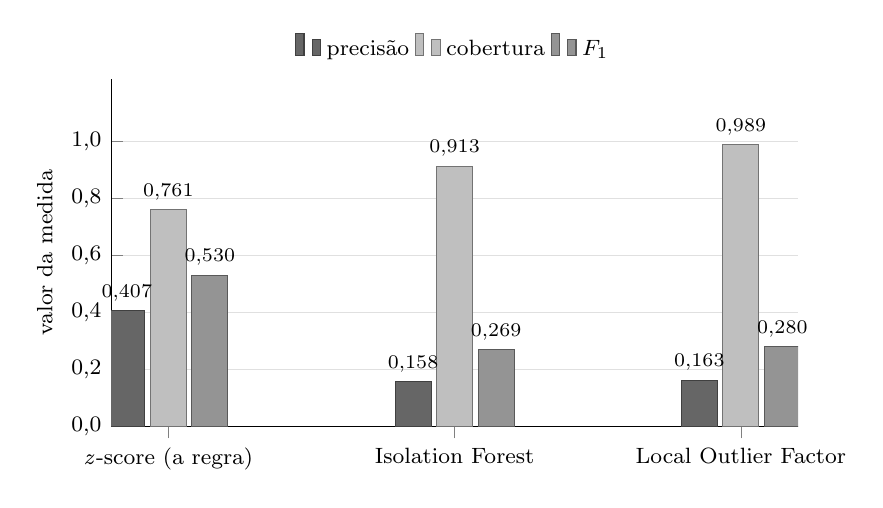
\begin{tikzpicture}
\begin{axis}[
  width=0.85\textwidth, height=6.0cm, ybar=2pt, bar width=13pt,
  ymin=0, ymax=1.22, ytick={0,0.2,0.4,0.6,0.8,1.0},
  yticklabels={{0,0},{0,2},{0,4},{0,6},{0,8},{1,0}},
  symbolic x coords={z, if, lof}, xtick={z, if, lof},
  xticklabels={\emph{z}-score (a regra), Isolation Forest, Local Outlier Factor},
  ylabel={valor da medida},
  legend style={at={(0.5,1.02)}, anchor=south, legend columns=3, font=\footnotesize, draw=none},
  nodes near coords, point meta=explicit symbolic,
  every node near coord/.append style={font=\scriptsize},
  tick label style={font=\footnotesize}, label style={font=\footnotesize},
  ymajorgrids, grid style={black!12}, axis lines*=left,
]
\addplot[fill=black!60, draw=black!75] coordinates {(z,0.407) [0,407] (if,0.158) [0,158] (lof,0.163) [0,163]};
\addplot[fill=black!25, draw=black!55] coordinates {(z,0.761) [0,761] (if,0.913) [0,913] (lof,0.989) [0,989]};
\addplot[fill=black!42, draw=black!65] coordinates {(z,0.530) [0,530] (if,0.269) [0,269] (lof,0.280) [0,280]};
\legend{precisão, cobertura, $F_1$}
\end{axis}
\end{tikzpicture}
\caption[A regra transparente contra dois detetores aprendidos]{Os três detetores sobre os mesmos
dados e sob o mesmo protocolo, restrito à região que os três conseguem pontuar. Os dois métodos
aprendidos assinalam quase tudo, com cobertura de $0{,}913$ e $0{,}989$, e acertam pouco, com
precisão em torno de $0{,}16$. A amplitude da taxa de disparo acompanha o mesmo padrão, com
$0{,}017$ para a regra contra $0{,}140$ e $0{,}183$ para os detetores aprendidos.}
\label{fig:av_detetores}
\end{figure}

A regra transparente supera os dois métodos, com quase o dobro do $F_1$ e com consistência entre
empresas substancialmente melhor. Este é o primeiro de três casos, ao longo do capítulo, em que uma
técnica mais sofisticada é comparada em condições equivalentes com uma técnica mais simples e não
obtém melhor resultado. A escolha do método simples passa assim a estar justificada por medição e
não por preferência.

A explicação não reside na qualidade dos métodos. Ambos determinam o que é invulgar a partir da geometria dos dados, por vias opostas. O
\emph{Isolation Forest} identifica o ponto raro pela facilidade com que sucessivos cortes
aleatórios o separam dos restantes \autocite{liu2008isolation}. O \emph{Local Outlier Factor}
confronta a densidade na vizinhança de cada ponto com a dos pontos que o rodeiam
\autocite{breunig2000lof}.

Trata-se de
métodos não paramétricos, exteriores à família estatística que \textcite{chandola2009anomaly}
caracteriza pela modelação da distribuição dos dados normais, e foram concebidos para conjuntos com
muitas variáveis em interação. O problema aqui tratado apresenta outra forma: uma série de retornos
por empresa, cuja estrutura pertinente é temporal. O agrupamento da volatilidade, formalizado pelos
modelos \gls{ARCH} e \gls{GARCH} \autocite{engle1982arch, bollerslev1986garch}, desloca ao longo do
tempo o limiar do que constitui um dia invulgar; uma janela deslizante acompanha essa deslocação
por construção, enquanto um detetor ajustado ao conjunto completo tem de a inferir.

Uma nota sobre a compatibilidade entre os valores: o \emph{z}-score aparece com $F_1 = 0{,}530$ nesta
comparação e com $0{,}516$ na anterior. Os dois valores medem o mesmo detetor sob protocolos
distintos. O segundo abrange todos os dias avaliados, enquanto o primeiro se restringe à região que
os três detetores conseguem pontuar, única em que a comparação entre eles é equitativa. A amplitude
segue a mesma regra, sendo $0{,}017$ neste protocolo e $0{,}015$ no anterior.

\subsection{Duas comparações que não confirmam as escolhas implantadas}

Duas experiências adicionais foram concebidas para justificar opções tomadas, e nenhuma delas as
confirmou. Ambas ficam reportadas tal como resultaram.

A primeira incide sobre o estimador de volatilidade. A alternativa a atribuir o mesmo peso aos vinte
dias da janela consiste em atribuir maior peso aos dias recentes, através de uma média com
decaimento exponencial. A Figura~\ref{fig:av_ewma} apresenta o resultado.

\begin{figure}[ht]
\centering
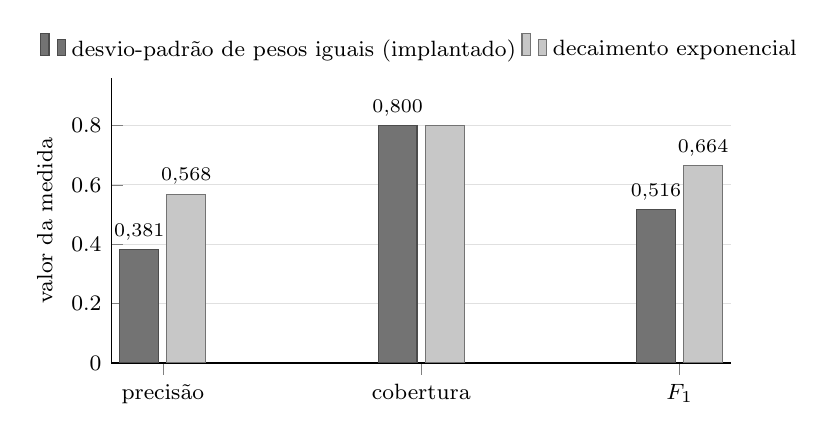
\begin{tikzpicture}
\begin{axis}[
  width=0.78\textwidth, height=5.2cm, ybar=3pt, bar width=14pt,
  ymin=0, ymax=0.96,
  symbolic x coords={p, c, f}, xtick={p, c, f},
  xticklabels={precisão, cobertura, $F_1$},
  ylabel={valor da medida},
  legend style={at={(0.5,1.02)}, anchor=south, legend columns=2, font=\footnotesize, draw=none},
  nodes near coords, point meta=explicit symbolic,
  every node near coord/.append style={font=\scriptsize},
  tick label style={font=\footnotesize}, label style={font=\footnotesize},
  ymajorgrids, grid style={black!12}, axis lines*=left,
]
\addplot[fill=black!55, draw=black!70] coordinates {(p,0.381) [0,381] (c,0.800) [0,800] (f,0.516) [0,516]};
\addplot[fill=black!22, draw=black!55] coordinates {(p,0.568) [0,568] (c,0.800) [] (f,0.664) [0,664]};
\legend{desvio-padrão de pesos iguais (implantado), decaimento exponencial}
\end{axis}
\end{tikzpicture}
\caption[Dois estimadores de volatilidade sobre o mesmo protocolo]{Os dois estimadores, com a mesma
cobertura. A alternativa com decaimento exponencial elimina quase metade dos falsos alarmes,
elevando a precisão de $0{,}381$ para $0{,}568$, e é ainda mais consistente entre empresas, com
amplitude de $0{,}012$ contra $0{,}015$. O sistema mantém o estimador que obteve o resultado
inferior, pela razão exposta no texto.}
\label{fig:av_ewma}
\end{figure}

Com cobertura idêntica, a alternativa obtém $F_1 = 0{,}664$ contra $0{,}516$ do estimador
implantado. O mecanismo é compreensível. Movimentos grandes ocorrem em grupo. Uma média de vinte dias com
pesos iguais dilui um choque por vinte observações e continua a assinalar os dias seguintes
durante semanas; uma média que privilegia o passado recente absorve-o de imediato.

O sistema mantém o estimador que obteve o resultado inferior. A razão é a que atravessa o trabalho:
a média e o desvio-padrão dos últimos vinte dias são explicáveis em duas frases a qualquer leitor, e
pesos com decaimento exponencial não o são. Numa ferramenta cujo argumento central é a
explicabilidade, um ganho de precisão obtido à custa da explicação não constitui inequivocamente um
ganho. Fica, porém, registado como escolha e não como resultado: a alternativa está medida, o ganho
está quantificado, e a sua adoção constitui uma alteração de pequena dimensão caso a explicabilidade
deixe de ser a restrição dominante.

A segunda experiência incide sobre a dimensão da janela, e a Figura~\ref{fig:av_janela} apresenta-a.

\begin{figure}[ht]
\centering
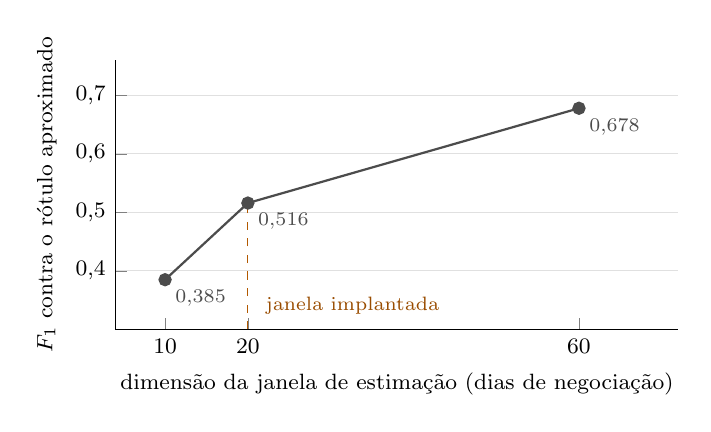
\begin{tikzpicture}
\begin{axis}[
  width=0.72\textwidth, height=5.0cm,
  xlabel={dimensão da janela de estimação (dias de negociação)},
  ylabel={$F_1$ contra o rótulo aproximado},
  xmin=4, xmax=72, ymin=0.30, ymax=0.76,
  xtick={10,20,60}, ytick={0.4,0.5,0.6,0.7},
  yticklabels={{0,4},{0,5},{0,6},{0,7}},
  tick label style={font=\footnotesize}, label style={font=\footnotesize},
  ymajorgrids, grid style={black!12}, axis lines*=left,
  nodes near coords, point meta=explicit symbolic,
  every node near coord/.append style={font=\scriptsize, anchor=north west},
]
\addplot[black!70, thick, mark=*, mark size=2pt]
  coordinates {(10,0.385) [0,385] (20,0.516) [0,516] (60,0.678) [0,678]};
\draw[dashed, orange!70!black] (axis cs:20,0.30) -- (axis cs:20,0.505);
\node[orange!60!black, font=\scriptsize, anchor=south west] at (axis cs:21,0.31) {janela implantada};
\end{axis}
\end{tikzpicture}
\caption[Ablação à dimensão da janela]{Desempenho contra o rótulo aproximado para três dimensões da
janela. O valor cresce de forma monótona com a dimensão da janela, e a janela implantada não é a que
obtém o melhor resultado. O texto expõe as duas razões pelas quais a janela mais longa não foi
adotada, sendo a segunda uma reserva sobre a validade desta própria medição.}
\label{fig:av_janela}
\end{figure}

Uma janela de sessenta dias obtém $F_1 = 0{,}678$ contra os $0{,}516$ da janela de vinte. Duas razões
justificam a manutenção da janela mais curta. A primeira é de responsividade: uma janela de sessenta
dias demora três meses a reagir a uma mudança de regime, e uma empresa que transite de calma a
volátil continuaria a ser julgada pela norma anterior.

A segunda respeita à validade desta medição
concreta. O rótulo é construído a partir do percentil de movimento da própria empresa, sendo por isso
relativo à volatilidade; uma janela mais longa produz uma norma menos adaptativa, que assinala com
maior frequência a cauda extrema, que é precisamente o que este rótulo premeia. Existe circularidade,
e ela favorece a janela longa por construção. Esta é a razão pela qual o argumento principal desta
secção é a consistência da taxa de disparo, que não recorre a rótulos. A formulação que subsiste é
que a janela de vinte dias foi escolhida por responsividade, e que a única medição existente sobre
este ponto não a sustenta.

\subsection{Limites da conclusão}

O rótulo é aproximado e relativo à volatilidade, razão pela qual o argumento de peso é o da
consistência, que dele não depende. As quinze empresas são todas de grande capitalização e foram
selecionadas em 2026, com a avaliação a percorrer o passado: sobreviveram por construção, e nenhuma
delas saiu de bolsa, foi absorvida ou desapareceu da lista. O que se mede é o comportamento do
método em empresas que subsistiram, e não na população de que foram extraídas. A comparação incide
ainda sobre este conjunto e este período, e nada nela permite antecipar o resultado noutro mercado
ou noutra década.

\section{Recuperação de precedentes}
\label{sec:av_qi2}

O segundo caso de estudo responde à \gls{QI}2: a recuperação por significado encontra notícias
passadas de outra empresa do mesmo setor melhor do que alternativas triviais. A resposta é
afirmativa nos cinco setores avaliados, e a formulação por setor é necessária, uma vez que o valor
agregado é enganador nos dois sentidos.

\subsection{Procedimento}

A avaliação de sistemas de recuperação enfrenta a ausência de uma lista de respostas corretas, dado
que nenhum conjunto de pares de notícias se encontra anotado como relacionado. Utiliza-se por isso
uma aproximação verificável: considera-se relevante a notícia recuperada que pertença ao mesmo setor
da notícia de consulta. A aproximação é imperfeita, porque duas notícias do mesmo setor podem tratar
de assuntos distintos, mas é objetiva e foi fixada antes de os resultados serem observados.

Impõe-se ainda uma restrição que torna a tarefa mais difícil: a notícia recuperada tem de pertencer a
uma empresa diferente. Sem ela, o sistema obteria bom desempenho devolvendo notícias da própria
empresa, que pertencem quase sempre ao mesmo setor por construção. O corpus contém $3\,714$ notícias
distribuídas por cinco setores, recolhidas ao longo de vinte e sete dias, e a medição utiliza
quinhentas consultas por repetição em cinco repetições com sementes distintas. A amplitude do corpus
delimita o que a medição estabelece: vinte e sete dias não sustentam afirmações sobre generalização
temporal. O protocolo não exige que o candidato seja anterior à consulta, e apenas $31{,}1\%$ dos vizinhos o
são. A verificação sob restrição causal foi feita em agregado sobre o corpus histórico, onde a
margem sobre o acaso se conserva, e não por setor.

\subsection{Resultado}

A Figura~\ref{fig:av_recuperacao} apresenta o método utilizado, uma variante de maior dimensão e as
alternativas triviais.

\begin{figure}[ht]
\centering
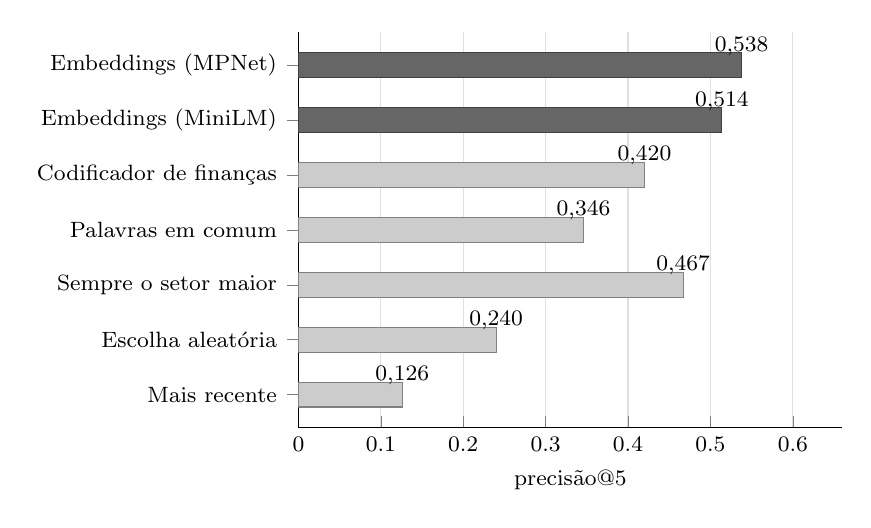
\begin{tikzpicture}
\begin{axis}[
  xbar, width=0.70\textwidth, height=6.6cm, bar width=9pt,
  xmin=0, xmax=0.66, enlarge y limits=0.10,
  symbolic y coords={rec, aleat, maior, lex, fin, mini, mpnet},
  ytick={rec, aleat, maior, lex, fin, mini, mpnet},
  yticklabels={Mais recente, Escolha aleatória, Sempre o setor maior, Palavras em comum,
               Codificador de finanças, Embeddings (MiniLM), Embeddings (MPNet)},
  nodes near coords, nodes near coords align={horizontal}, point meta=explicit symbolic,
  every node near coord/.append style={font=\footnotesize},
  xlabel={precisão@5},
  tick label style={font=\footnotesize}, label style={font=\footnotesize},
  xmajorgrids, grid style={black!12}, axis lines*=left,
]
\addplot[bar shift=0pt, fill=black!20, draw=black!50] coordinates {
  (0.126,rec) [0,126] (0.240,aleat) [0,240] (0.467,maior) [0,467] (0.346,lex) [0,346]
  (0.420,fin) [0,420]};
\addplot[bar shift=0pt, fill=black!60, draw=black!75] coordinates {
  (0.514,mini) [0,514] (0.538,mpnet) [0,538]};
\end{axis}
\end{tikzpicture}
\caption[Recuperação: o método contra cinco alternativas]{Precisão@5 do método utilizado, a escuro,
contra cinco alternativas. As barras claras incluem duas linhas de base triviais, uma linha lexical e
um codificador específico do domínio financeiro. A alternativa de devolver sempre notícias do setor
maior obtém $0{,}467$ sem qualquer modelo, valor discutido no texto e que obriga a ler o agregado
com reserva.}
\label{fig:av_recuperacao}
\end{figure}

A escolha aleatória acerta em $24{,}0\%$ dos casos, e é esse o valor de referência, e não zero, uma
vez que os setores existem em número finito e têm dimensões distintas. A procura por palavras em
comum eleva o resultado para $34{,}6\%$, e a comparação de significado para $51{,}4\%$.

A linha lexical corresponde à forma mais simples dessa família: contagem de palavras projetada por
dispersão e comparada pelo cosseno, sem ponderação pela raridade dos termos, sem saturação da
frequência e sem normalização pelo comprimento do texto. Pertence à tradição que vai do modelo de
espaço vetorial \autocite{salton1975vsm} às funções de ordenação probabilísticas como o BM25
\autocite{robertson2009bm25}, situando-se no degrau inicial dessa família. Os dezassete pontos
percentuais que a representação de frases \autocite{reimers2019sbert} acrescenta medem, por
conseguinte, a distância a um ponto de partida elementar e não a distância a um sistema lexical
afinado. A comparação com uma função de ordenação bem parametrizada constitui trabalho por realizar,
e é a que tornaria esta conclusão mais forte.

O codificador específico do domínio financeiro obtém $0{,}420$, o valor mais baixo de todos os
modelos avaliados. O modelo avaliado é o ponto de controlo público \texttt{ProsusAI/finbert},
identificado desta forma por ser o artefacto exato sobre o qual a medição incide; pertence à
família de codificadores financeiros de que \textcite{liu2020finbert} e \textcite{huang2023finbert}
são as versões documentadas em publicações revistas por pares. Foi utilizado com a média dos seus vetores como
representação da frase, que é a forma de o aplicar sem novo treino. Trata-se de um codificador
ajustado para classificação de sentimento e não para posicionar frases num espaço onde a distância
signifique semelhança, e é precisamente esse objetivo de treino que o Sentence-BERT acrescenta
\autocite{reimers2019sbert}. A medição estabelece que este modelo de domínio, utilizado desta forma,
obtém resultado inferior a um modelo genérico treinado para semelhança; não estabelece que
conhecimento de domínio seja irrelevante para a tarefa.

\subsection{A alternativa trivial que o valor agregado esconde}

O corpus não está equilibrado: $1\,736$ das $3\,714$ notícias, quase metade, pertencem ao setor da
tecnologia. Existe por isso uma estratégia que dispensa qualquer modelo e não observa sequer a
consulta, consistindo em devolver invariavelmente cinco notícias de tecnologia. Acerta em todas as
consultas de tecnologia e em nenhuma das restantes, pelo que a sua precisão iguala exatamente a
fração de consultas que são de tecnologia, $0{,}467$. Medida contra esta alternativa, e não contra o
acaso uniforme, a margem do método reduz-se de $+0{,}274$ para $+0{,}047$, e a linha lexical de
$0{,}346$ passa a situar-se abaixo do valor de referência.

O valor agregado é, contudo, o elemento enganador, e não o método. A estratégia trivial obtém
$1{,}000$ nas consultas de tecnologia e $0{,}000$ em todas as outras, devolvendo notícias de
semicondutores a quem consulta sobre uma petrolífera. O que ela explora não é uma propriedade do
problema, mas a composição deste corpus.

A comparação que resiste a esta objeção é a que se realiza dentro de cada setor, onde a estratégia
trivial não tem por onde se apoiar. O painel A da Figura~\ref{fig:av_setor_causal} apresenta-a.

\begin{figure}[ht]
\centering

\includegraphics[width=0.96\textwidth]{figures/eval_retrieval_sector_causal.pdf}
\caption[Recuperação por setor e sob a restrição temporal]{Em A, a precisão@5 e o valor de acaso
correspondente dentro de cada setor: o método situa-se acima do respetivo valor de referência nos
cinco. Em B, o protocolo simétrico do teste de escala e o protocolo causal que reproduz a restrição
da produção, cada um ao lado do seu valor de referência. A precisão desce de $0{,}595$ para
$0{,}513$, mas a margem sobre o acaso varia apenas de $+0{,}262$ para $+0{,}254$.}
\label{fig:av_setor_causal}
\end{figure}

O valor de acaso é de $0{,}429$ na tecnologia e situa-se em torno de $0{,}072$ em cada um dos quatro
setores restantes. O método obtém $0{,}712$ na tecnologia, $0{,}448$ na energia, $0{,}419$ na saúde,
$0{,}272$ na banca e $0{,}171$ no consumo. Onde o valor agregado é dominado, o método acrescenta
$0{,}283$; onde o corpus é escasso, obtém várias vezes o valor de referência. O agregado subestima o
método e sobrestima a alternativa trivial pela mesma razão, que é a de quase metade das consultas
provir do único setor onde o valor de referência já era elevado. A afirmação que o trabalho sustenta
é por isso a mais estreita: a recuperação semântica supera a taxa-base dentro de cada um dos cinco
setores, e o valor agregado não é a forma adequada de o enunciar.

A variante de maior dimensão obtém $0{,}538 \pm 0{,}011$ contra $0{,}514 \pm 0{,}015$ da utilizada,
sobre cinco sementes; a diferença é pequena face à dispersão e nenhum teste de significância foi
realizado. Dois codificadores mais recentes obtêm $0{,}504$ e $0{,}513$, indistinguíveis do
implantado. A adoção do modelo
mais pequeno em produção decorreu do custo computacional e não de uma vantagem de qualidade,
constituindo uma troca explícita cujo preço em precisão está quantificado. A alternativa aparentemente mais
razoável, que consiste em apresentar as notícias mais recentes, obtém $0{,}126$, o valor mais baixo
de todos, o que é coerente com a ausência de qualquer razão para a notícia mais recente sobre outra
empresa estar relacionada com a notícia em análise.

\subsection{Comportamento à escala e sob a restrição da produção}

A avaliação anterior incide sobre um corpus recente e de dimensão limitada. Para verificar que o
resultado não depende desse corpus, a mesma medição foi repetida sobre o conjunto histórico
completo, com aproximadamente oitenta mil notícias de seis anos. Neste protocolo simétrico, que
ainda admite candidatos posteriores à consulta, a precisão@5 sobe para $0{,}595$. A subida não deve,
porém, ser lida na íntegra como ganho: o valor de acaso sobe igualmente, de $0{,}240$ para $0{,}333$,
porque a composição por setores é distinta. Medida contra o valor de referência respetivo, a margem
é de $+0{,}274$ no primeiro caso e de $+0{,}262$ no segundo. O resultado estabelece que o método não
se degrada quando o corpus passa de recente e curto para seis anos, e não que melhore com mais dados.

O protocolo anterior concede uma liberdade que o sistema em produção não possui. A única restrição
imposta é a de o candidato pertencer a outra empresa, o que permite que seja posterior à consulta, e
esse caso é comum: no corpus recente, $38{,}7\%$ dos vizinhos devolvidos têm data posterior à da
consulta e outros $30{,}2\%$ são do mesmo dia. O sistema implantado não dispõe dessa liberdade, uma
vez que a base de precedentes só recebe um caso oito dias após a sua observação, conforme a
Secção~\ref{sec:sis_base} descreve.

Não é utilização de informação futura no sentido corrente. O critério de acerto é a pertença ao
mesmo setor, e o setor de uma notícia não varia com o tempo, pelo que a direção temporal não pode
inflacionar a precisão. O que está em causa é a correspondência
entre o valor reportado e a tarefa que a questão de investigação descreve, que fala em notícias
passadas. A medição repete o protocolo acrescentando à máscara a condição de o candidato ser
estritamente anterior à consulta, e reproduz o valor simétrico na mesma execução para que a
comparação seja emparelhada. Nenhuma das $2\,500$ consultas ficou sem passado suficiente. O
resultado consta do painel B da Figura~\ref{fig:av_setor_causal}: a precisão desce $0{,}082$, o valor
de referência desce quase outro tanto, e a margem varia $0{,}008$. O método conserva praticamente
toda a vantagem quando obrigado a operar como opera em produção.

Esta é a terceira ocasião no capítulo em que a leitura de uma precisão sem o valor de referência
correspondente conduziria à conclusão errada. Sucedeu na passagem do corpus recente para o completo,
sucede na precisão dentro do orçamento tratada na Secção~\ref{sec:av_qi3}, e sucede aqui. A precisão
é uma quantidade sem significado próprio, que apenas o adquire ao lado da alternativa sem informação.

\subsection{Limites da conclusão}

A pertença ao mesmo setor não equivale a relação entre notícias, sendo uma aproximação construída por
ser verificável e não por corresponder exatamente à propriedade pretendida.

A segunda observação tem consequências para o produto: a recuperação capta tema e não direção. Duas
notícias podem tratar do mesmo assunto e o preço evoluir em sentidos opostos, que foi o que sucedeu
no exemplo apresentado no Capítulo~\ref{cap:sistema}. A Figura~\ref{fig:av_direcao} quantifica-o.

\begin{figure}[ht]
\centering
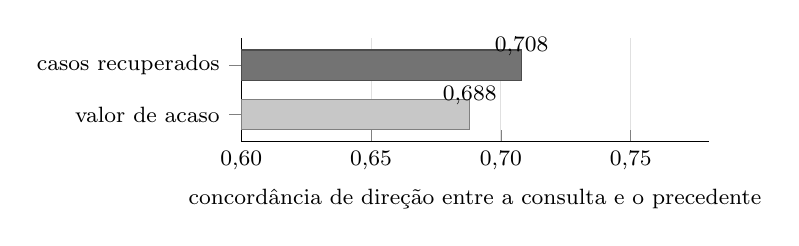
\begin{tikzpicture}
\begin{axis}[
  xbar, width=0.62\textwidth, height=2.9cm, bar width=11pt,
  xmin=0.60, xmax=0.78, enlarge y limits=0.55,
  symbolic y coords={acaso, metodo}, ytick={acaso, metodo},
  yticklabels={valor de acaso, casos recuperados},
  nodes near coords, nodes near coords align={horizontal}, point meta=explicit symbolic,
  every node near coord/.append style={font=\footnotesize},
  xlabel={concordância de direção entre a consulta e o precedente},
  xtick={0.60,0.65,0.70,0.75}, xticklabels={{0,60},{0,65},{0,70},{0,75}},
  tick label style={font=\footnotesize}, label style={font=\footnotesize},
  xmajorgrids, grid style={black!12}, axis lines*=left,
]
\addplot[bar shift=0pt, fill=black!22, draw=black!50] coordinates {(0.688,acaso) [0,688]};
\addplot[bar shift=0pt, fill=black!55, draw=black!70] coordinates {(0.708,metodo) [0,708]};
\end{axis}
\end{tikzpicture}
\caption[Tema e direção não são a mesma propriedade]{Fração de casos recuperados cujo preço evoluiu
no mesmo sentido que o da notícia de consulta, contra o valor obtido por emparelhamento aleatório sob
as mesmas restrições. A diferença é de $0{,}020$. O sistema apresenta por isso os casos
individualmente, e o texto do alerta declara que a semelhança é de tema.}
\label{fig:av_direcao}
\end{figure}

A concordância de direção entre a notícia de consulta e os casos recuperados situa-se em $0{,}708$
contra um valor de acaso de $0{,}688$. É por esta razão que o sistema apresenta os casos um a um e
nunca os resume a uma média, que seria lida como previsão, e que o texto do alerta declara
explicitamente tratar-se de casos semelhantes quanto ao tema.

\section{Triagem de notícias}
\label{sec:av_qi3}

O terceiro caso de estudo responde à \gls{QI}3: um modelo treinado prioriza notícias melhor do que
uma linha de base baseada apenas em volatilidade. A resposta é negativa, e é o resultado com maior
valor informativo do trabalho.

\subsection{Procedimento}

O conjunto de dados contém $79\,753$ exemplos entre 2018 e 2023, cada um correspondente a uma notícia
com o contexto de mercado do dia e o rótulo definido na Secção~\ref{sec:met_triagem}. A divisão é
cronológica com embargo, e a prevalência de casos positivos no bloco de teste é de $0{,}378$. A
métrica principal é a \gls{PRAUC}, adequada quando as duas classes estão desequilibradas.

Para efeitos práticos, uma diferença de \gls{PRAUC} inferior a $0{,}02$ é tratada como
indistinguível, mesmo quando o intervalo emparelhado exclui zero. O limite é uma escolha do autor,
declarada antes dos resultados, o que obriga à sua aplicação nos dois sentidos.

Dois cuidados de montagem asseguram que a comparação não favorece a conclusão obtida. O primeiro é a
inclusão de um conjunto de árvores treinado por reforço do gradiente \autocite{friedman2001gbm}, o
mais expressivo dos modelos comparados, por captar interações e efeitos não lineares que a regressão
logística não capta por construção. Este modelo foi executado com os parâmetros por defeito da
biblioteca, sem procura de hiperparâmetros, o que limita o alcance da sua derrota: estabelece que o
texto não produz vantagem nesta montagem, e não que a não produziria num modelo não linear afinado.
O segundo cuidado é a conversão de todas as pontuações em probabilidades por calibração \emph{a
posteriori} sobre um bloco de validação reservado \autocite{niculescu2005calibration}, sem a qual a
comparação pelo índice de Brier não seria válida entre modelos.

Uma entrada não está disponível no mesmo referencial em produção. O retorno do próprio dia
corresponde, no conjunto histórico, ao movimento completo do dia da notícia, ao passo que em produção
a notícia é pontuada antes de esse dia encerrar. O resultado apresentado avalia por isso o modelo com
a variável diária completa e não demonstra paridade com a pontuação intradiária. A direção da assimetria é conhecida. A entrada em causa pertence ao bloco de contexto, presente
nos modelos de resultado inferior. A linha de base vencedora usa uma só entrada: a volatilidade
dos vinte dias anteriores, fechada na véspera. O referencial mais generoso
encontra-se do lado dos modelos que a comparação não favorece, e a sua correção só poderia tornar o
resultado negativo mais forte.

\subsection{Resultado}

A Figura~\ref{fig:av_triagem} apresenta os seis modelos comparados. As curvas completas de
precisão e cobertura, de que estes valores agregados são a área, constam dos artefactos de
avaliação identificados no Apêndice~\ref{ap:reprodutibilidade}; nelas a curva do modelo de
volatilidade situa-se acima das restantes em quase toda a extensão do eixo, o que estabelece que a
diferença não é um artefacto do valor agregado.

\begin{figure}[ht]
\centering
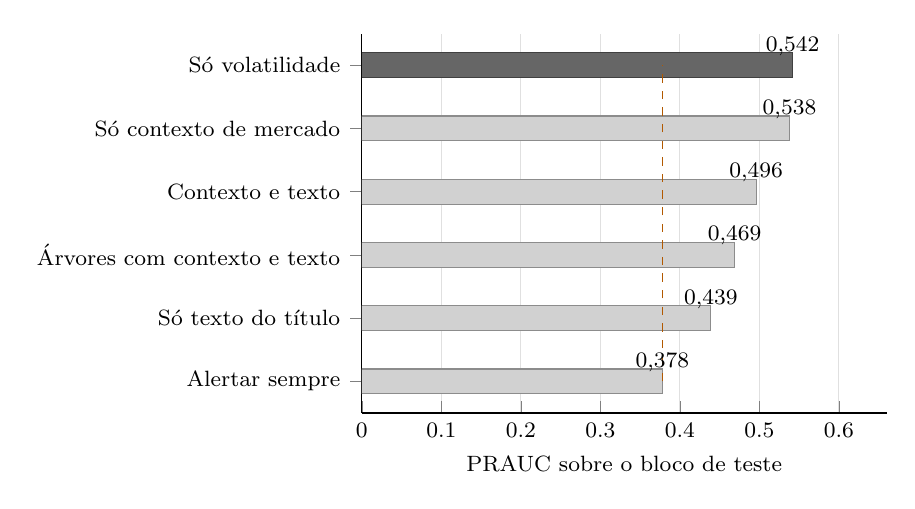
\begin{tikzpicture}
\begin{axis}[
  xbar, width=0.68\textwidth, height=6.4cm, bar width=9pt,
  xmin=0, xmax=0.66, enlarge y limits=0.10,
  symbolic y coords={sempre, texto, gbm, ctxtexto, ctx, vol},
  ytick={sempre, texto, gbm, ctxtexto, ctx, vol},
  yticklabels={Alertar sempre, Só texto do título, Árvores com contexto e texto,
               Contexto e texto, Só contexto de mercado, Só volatilidade},
  nodes near coords, nodes near coords align={horizontal}, point meta=explicit symbolic,
  every node near coord/.append style={font=\footnotesize},
  xlabel={\gls{PRAUC} sobre o bloco de teste},
  tick label style={font=\footnotesize}, label style={font=\footnotesize},
  xmajorgrids, grid style={black!12}, axis lines*=left,
]
\addplot[bar shift=0pt, fill=black!18, draw=black!45] coordinates {
  (0.378,sempre) [0,378] (0.439,texto) [0,439] (0.469,gbm) [0,469] (0.496,ctxtexto) [0,496]
  (0.538,ctx) [0,538]};
\addplot[bar shift=0pt, fill=black!60, draw=black!75] coordinates {(0.542,vol) [0,542]};
\draw[dashed, orange!70!black] (axis cs:0.378,sempre) -- (axis cs:0.378,vol);
\end{axis}
\end{tikzpicture}
\caption[Seis modelos de triagem sobre o mesmo bloco de teste]{Área sob a curva de precisão e
cobertura dos seis modelos. A linha tracejada assinala a prevalência do bloco de teste, que é o valor
obtido por um modelo que atribua a mesma probabilidade a todos os exemplos. Os valores são pontos, e
os intervalos marginais a noventa e cinco por cento, obtidos por reamostragem dos $1\,951$ grupos,
são amplos e sobrepõem-se: $[0{,}492;\,0{,}597]$ para a volatilidade, $[0{,}487;\,0{,}592]$ para o
contexto e $[0{,}453;\,0{,}540]$ para o contexto com texto. A comparação que a subsecção seguinte
sustenta é a diferença emparelhada entre modelos sobre as mesmas reamostragens, e não a distância
entre dois pontos.}
\label{fig:av_triagem}
\end{figure}


O valor mais elevado pertence ao modelo mais simples de todos, o que utiliza apenas a volatilidade
recente. Acrescentar-lhe o restante contexto não altera o resultado de forma distinguível, com
$0{,}538$ contra $0{,}542$; acrescentar o texto do título deteriora-o de forma distinguível, com
$0{,}496$. O índice de Brier acompanha a mesma ordenação, com $0{,}218$ para o modelo de
volatilidade contra $0{,}229$ para o modelo com texto e $0{,}622$ para o modelo que anuncia sempre a
unidade. A hipótese inicial, segundo a qual o texto da notícia traria informação ausente dos preços,
não é confirmada sobre este corpus.

\subsection{Três verificações à montagem experimental}

O resultado negativo foi submetido a três verificações destinadas a determinar se decorre da montagem
experimental.

A primeira respeita ao ajuste do modelo de texto. A comparação foi repetida concedendo ao texto as
melhores condições disponíveis, com regularização afinada, redução do bloco de texto a trinta e duas
dimensões e um modelo de linguagem especializado em finanças. O melhor resultado do texto sobe para
$0{,}533$ e permanece abaixo dos $0{,}542$ da volatilidade.

A segunda respeita ao ruído de amostragem. O bloco de teste foi reamostrado mil vezes por grupos
constituídos pela empresa e pelo dia, uma vez que notícias do mesmo dia sobre a mesma empresa
partilham o rótulo e não constituem observações independentes. A diferença entre a volatilidade e a
variante com texto é de $+0{,}048$, com intervalo entre $+0{,}032$ e $+0{,}066$, que exclui zero e
supera o limite prático de $0{,}02$. É a única comparação desta secção que o supera.

O alcance deste
intervalo é, contudo, limitado: a reamostragem realiza-se dentro de
um único bloco de teste, com duzentos e vinte e um dias de negociação, pelo que mede o ruído de
amostragem nesse período e nada estabelece sobre a estabilidade entre períodos. A distinção não é
teórica neste trabalho, dado que a Secção~\ref{sec:av_producao} reporta um deslocamento significativo
na distribuição da entrada principal. Uma origem rolante com três ou quatro cortes sucessivos
responderia à pergunta mais larga, e não foi realizada.

A terceira respeita à definição do rótulo, que utiliza um limiar de dois por cento e um horizonte de
três dias, ambos escolhidos pelo autor. A comparação foi repetida para nove combinações de limiar e
horizonte, e a Figura~\ref{fig:av_rotulos} apresenta o resultado.

\begin{figure}[ht]
\centering
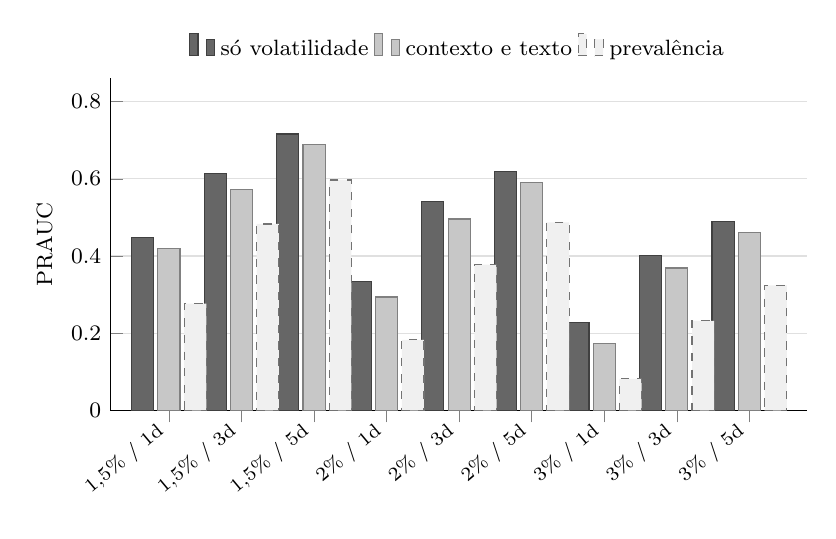
\begin{tikzpicture}
\begin{axis}[
  width=0.86\textwidth, height=5.8cm, ybar=1.5pt, bar width=8pt,
  ymin=0, ymax=0.86,
  symbolic x coords={a,b,c,d,e,f,g,h,i}, xtick={a,b,c,d,e,f,g,h,i},
  xticklabels={{1,5\% / 1d},{1,5\% / 3d},{1,5\% / 5d},{2\% / 1d},{2\% / 3d},{2\% / 5d},
               {3\% / 1d},{3\% / 3d},{3\% / 5d}},
  xticklabel style={rotate=40, anchor=east, font=\scriptsize},
  ylabel={\gls{PRAUC}},
  legend style={at={(0.5,1.02)}, anchor=south, legend columns=3, font=\footnotesize, draw=none},
  tick label style={font=\footnotesize}, label style={font=\footnotesize},
  ymajorgrids, grid style={black!12}, axis lines*=left,
]
\addplot[fill=black!60, draw=black!75] coordinates {
  (a,0.449) (b,0.613) (c,0.716) (d,0.334) (e,0.542) (f,0.620) (g,0.228) (h,0.402) (i,0.489)};
\addplot[fill=black!22, draw=black!50] coordinates {
  (a,0.420) (b,0.572) (c,0.689) (d,0.294) (e,0.496) (f,0.590) (g,0.174) (h,0.369) (i,0.461)};
\addplot[fill=black!6, draw=black!55, dashed] coordinates {
  (a,0.277) (b,0.483) (c,0.597) (d,0.183) (e,0.378) (f,0.487) (g,0.082) (h,0.232) (i,0.324)};
\legend{só volatilidade, contexto e texto, prevalência}
\end{axis}
\end{tikzpicture}
\caption[O resultado sob nove definições alternativas de rótulo]{Desempenho das duas famílias sob
nove combinações de limiar e horizonte, com a prevalência de cada célula como referência. A
volatilidade iguala ou supera o modelo com texto nas nove combinações, com prevalências entre
$0{,}082$ e $0{,}597$. A célula correspondente ao rótulo utilizado no restante capítulo é a quinta,
com limiar de dois por cento e horizonte de três dias.}
\label{fig:av_rotulos}
\end{figure}

O resultado negativo resiste às três verificações. A volatilidade iguala ou supera o modelo com texto
nas nove definições de rótulo, com prevalências entre $0{,}082$ e $0{,}597$, o que retira à escolha
concreta de limiar e horizonte o estatuto de ponto de ataque.

Uma quarta verificação incide sobre a composição dos blocos e conduz a uma conclusão que atua nos
dois sentidos. Os três blocos quase não partilham empresas. O bloco de treino decorre entre 2 de
janeiro de 2018 e 3 de março de 2022 e contém treze empresas; o bloco de teste decorre entre 2 de
fevereiro e 18 de dezembro de 2023 e contém nove. Cinco empresas do treino não figuram uma única vez
no teste, e uma empresa do teste, responsável por $17{,}1\%$ das suas linhas, nunca figura no treino.
Para as empresas presentes em ambos os lados, a taxa de positivos desloca-se de forma acentuada, e a
Apple passa de $0{,}448$ no treino para $0{,}183$ no teste. Estes valores leem-se diretamente das
colunas de identificação e de bloco do conjunto congelado e não exigem qualquer execução adicional.

Não se trata de utilização de informação futura nem de erro de divisão: o corte é realizado por dia,
e a proporção respeita a definida na Secção~\ref{sec:met_triagem}. É a composição do corpus que varia
com o tempo, pela mesma razão que torna o bloco de teste maior do que o de treino, uma vez que as
empresas sobre as quais se escreve em 2018 não são as mesmas de 2023.

A favor do resultado negativo pesa o seguinte. O sinal do modelo é essencialmente a identidade da
empresa, conforme a Secção~\ref{sec:av_ablacao} estabelece, e essa identidade é estimada sobre um
conjunto de empresas quase ausente do bloco onde é avaliada. A volatilidade dos vinte dias
anteriores, fechada na véspera, é comparável entre empresas e não depende da identidade de
nenhuma. Contra o
resultado, a comparação não separa a hipótese de o modelo ser pior da hipótese de a identidade não
transferir entre estes dois períodos, separação que exigiria uma divisão de composição constante. A
mesma constatação explica, sem recurso ao acaso, a prevalência de $47{,}0\%$ da validação contra
$37{,}8\%$ do teste, que correspondem a conjuntos de empresas distintos e não apenas a períodos
distintos.

\subsection{Utilidade sob a restrição de orçamento}

O produto apresenta no máximo cinco alertas por dia, pelo que a pergunta com significado operacional
é a de qual a fração de acertos entre as cinco notícias escolhidas em cada dia. A
Figura~\ref{fig:av_orcamento} apresenta quatro formas de as escolher.

\begin{figure}[ht]
\centering
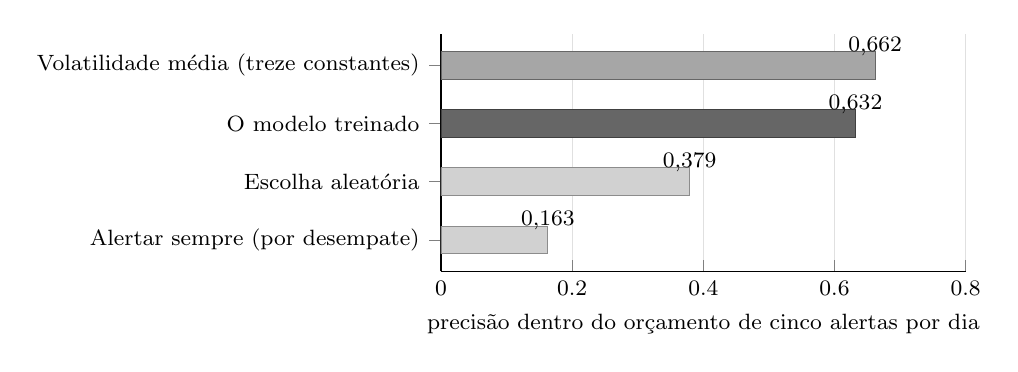
\begin{tikzpicture}
\begin{axis}[
  xbar, width=0.68\textwidth, height=4.6cm, bar width=10pt,
  xmin=0, xmax=0.80, enlarge y limits=0.18,
  symbolic y coords={alfa, acaso, modelo, volat},
  ytick={alfa, acaso, modelo, volat},
  yticklabels={Alertar sempre (por desempate), Escolha aleatória, O modelo treinado,
               Volatilidade média (treze constantes)},
  nodes near coords, nodes near coords align={horizontal}, point meta=explicit symbolic,
  every node near coord/.append style={font=\footnotesize},
  xlabel={precisão dentro do orçamento de cinco alertas por dia},
  tick label style={font=\footnotesize}, label style={font=\footnotesize},
  xmajorgrids, grid style={black!12}, axis lines*=left,
]
\addplot[bar shift=0pt, fill=black!18, draw=black!45] coordinates {(0.163,alfa) [0,163] (0.379,acaso) [0,379]};
\addplot[bar shift=0pt, fill=black!60, draw=black!75] coordinates {(0.632,modelo) [0,632]};
\addplot[bar shift=0pt, fill=black!35, draw=black!60] coordinates {(0.662,volat) [0,662]};
\end{axis}
\end{tikzpicture}
\caption[Precisão dentro de um orçamento de cinco alertas por dia]{Quatro formas de escolher as cinco
notícias do dia, sobre o mesmo bloco de teste. A primeira barra não mede escolha às cegas, pela razão
exposta no texto; o valor que corresponde à escolha às cegas é o segundo, $0{,}379 \pm 0{,}017$ sobre
quarenta sementes. As quatro políticas escolhem conhecendo o dia completo, pelo que os valores são
limites superiores do que uma política em linha consegue obter.}
\label{fig:av_orcamento}
\end{figure}

A primeira barra exige uma explicação, uma vez que a sua designação induz em erro. O modelo que
alerta sempre atribui a mesma pontuação a todas as notícias, e quando todas empatam a métrica
seleciona pela ordem em que as linhas surgem no ficheiro, que está ordenado por data e por nome da
empresa. Esse valor de $0{,}163$ mede a escolha por ordem alfabética e não a escolha aleatória, e
todas as linhas que seleciona pertencem à empresa que ocupa a primeira posição no alfabeto. Comparado
com o valor de referência correto, o ganho do modelo é de $1{,}67$ vezes e não das quase quatro vezes
que a primeira leitura sugeriria. A lição é geral e aplica-se ao restante capítulo: verificar o que a
linha de base mede é tão necessário quanto verificar o que o modelo faz.

A terceira e a quarta barras contêm o resultado incómodo. Uma tabela de treze constantes,
correspondentes à volatilidade média de cada empresa, calculada exclusivamente sobre o bloco de
treino e sem leitura de um único título, obtém $0{,}662$ e supera o modelo treinado. A comparação
tem uma reserva que a torna menos limpa do que parece: $17{,}1\%$ das linhas do bloco de teste
pertencem a uma empresa ausente do treino e recebem a mediana global em vez de uma constante
própria. É, ainda assim, o terceiro caso do capítulo em que o método mais simples obtém melhor
resultado. O que a evidência sustenta é
que ordenar por volatilidade compensa, e não que aprender compense.

\subsection{Ablação das entradas do modelo}
\label{sec:av_ablacao}

O resultado anterior sugere que o modelo implantado reconhece a empresa e não a notícia. A
verificação dessa hipótese consiste em tentar reproduzi-lo com uma tabela de consulta que atribua a
cada empresa um único número fixado no bloco de treino, correspondente à fração das suas notícias que
se revelaram materiais. Essa tabela não observa o título, não observa o dia e devolve invariavelmente
o mesmo valor para a mesma empresa. A Figura~\ref{fig:av_ablacao} compara-a com o modelo implantado e
desmonta o modelo entrada a entrada, sob o protocolo congelado.

\begin{figure}[ht]
\centering
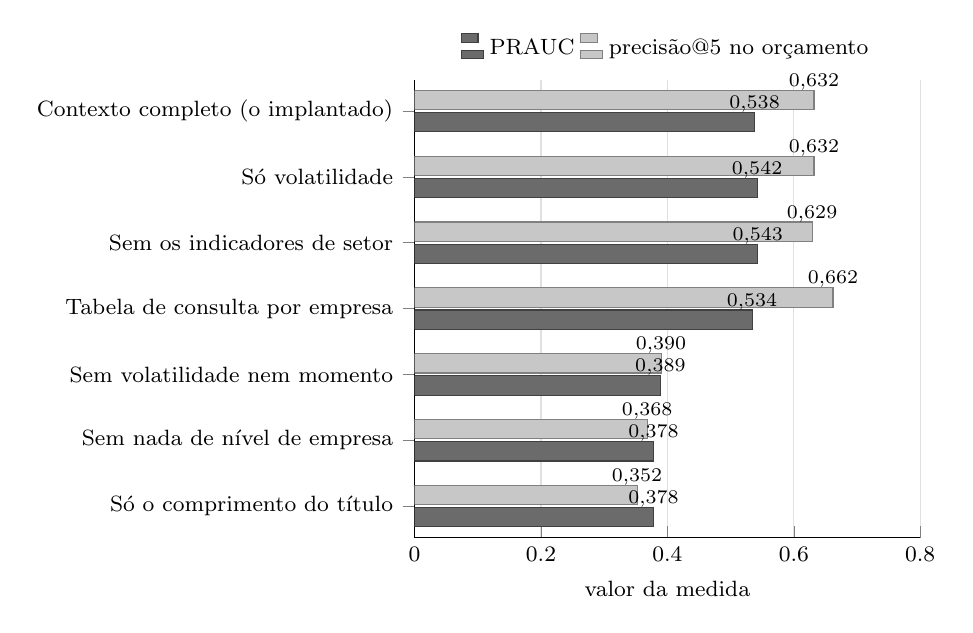
\begin{tikzpicture}
\begin{axis}[
  xbar=1pt, width=0.66\textwidth, height=7.4cm, bar width=7pt,
  xmin=0, xmax=0.80, enlarge y limits=0.08,
  symbolic y coords={comp, nada, semvol, tabela, semset, vol, ctx},
  ytick={comp, nada, semvol, tabela, semset, vol, ctx},
  yticklabels={Só o comprimento do título, Sem nada de nível de empresa,
               Sem volatilidade nem momento, Tabela de consulta por empresa,
               Sem os indicadores de setor, Só volatilidade,
               Contexto completo (o implantado)},
  legend style={at={(0.5,1.02)}, anchor=south, legend columns=2, font=\footnotesize, draw=none},
  nodes near coords, nodes near coords align={horizontal}, point meta=explicit symbolic,
  every node near coord/.append style={font=\scriptsize},
  xlabel={valor da medida},
  tick label style={font=\footnotesize}, label style={font=\footnotesize},
  xmajorgrids, grid style={black!12}, axis lines*=left,
]
\addplot[fill=black!58, draw=black!75] coordinates {
  (0.378,comp) [0,378] (0.378,nada) [0,378] (0.389,semvol) [0,389] (0.534,tabela) [0,534]
  (0.543,semset) [0,543] (0.542,vol) [0,542] (0.538,ctx) [0,538]};
\addplot[fill=black!22, draw=black!50] coordinates {
  (0.352,comp) [0,352] (0.368,nada) [0,368] (0.390,semvol) [0,390] (0.662,tabela) [0,662]
  (0.629,semset) [0,629] (0.632,vol) [0,632] (0.632,ctx) [0,632]};
\legend{\gls{PRAUC}, precisão@5 no orçamento}
\end{axis}
\end{tikzpicture}
\caption[O modelo desmontado entrada a entrada]{Cada linha corresponde a um modelo treinado com menos
informação do que o anterior. A linha decisiva é a da tabela de consulta, que não observa a notícia e
iguala o modelo implantado na primeira medida e o supera na segunda. As duas linhas inferiores, que
não dispõem de qualquer entrada de nível de empresa, situam-se exatamente na prevalência do bloco de
teste.}
\label{fig:av_ablacao}
\end{figure}

Três leituras resultam da figura, e nenhuma depende de interpretação.

A tabela de consulta iguala o modelo e supera-o numa das medidas. Na \gls{PRAUC} obtém $0{,}534$
contra $0{,}538$, uma diferença de $0{,}004$; na precisão dentro do orçamento, que é a medida mais
próxima da utilização real, obtém $0{,}662$ contra $0{,}632$. Esta segunda diferença não foi
acompanhada de reamostragem por grupos, ao contrário das diferenças de \gls{PRAUC} desta secção, pelo
que se reporta como observação e não como superioridade estabelecida. Um número por empresa, fixado
meses antes e nunca atualizado, produz o mesmo efeito que o modelo treinado.

Sem as entradas de nível de empresa não subsiste sinal. Retirando-as, a \gls{PRAUC} desce para
$0{,}378$, que é precisamente a prevalência do bloco de teste e o valor definido na
Secção~\ref{sec:av_desenho} como correspondente à ausência de informação.

A única entrada que descreve a notícia nada acrescenta. O comprimento do título, isoladamente,
produz igualmente $0{,}378$, o que torna a única informação por título recebida pelo modelo
implantado indistinguível da ausência de informação.

Estas leituras obrigam a separar duas afirmações. A conclusão científica da \gls{QI}3 mantém-se: a
variante com texto dispõe de trezentos e oitenta e quatro números por título, possuindo por isso
informação real sobre a notícia, e ainda assim obteve $0{,}496$ contra os $0{,}542$ da volatilidade,
sendo essa a comparação que responde à questão. A decisão de produto, por seu turno, estava errada
por razão distinta: o que foi implantado como porta de decisão foi a variante sem texto, escolhida
por uma métrica que não formulava a pergunta de que o produto necessitava.

A manutenção da variante de nove entradas não decorre de esta apresentar o melhor valor entre as que
cabiam no contentor de execução. Pelo critério fixado antes dos resultados, quatro valores são indistinguíveis entre si: os
$0{,}542$ da volatilidade, os $0{,}543$ da variante sem indicadores de setor, os $0{,}538$ da
variante implantada e os $0{,}534$ da tabela de consulta. As diferenças situam-se entre $0{,}004$
e $0{,}009$, muito abaixo do limite de $0{,}02$. Aplicar esse limite apenas quando desfavorece uma
conclusão seria não o ter fixado. A única diferença que o
critério separa nesta comparação é a que distingue estas quatro variantes do bloco com texto, de
$+0{,}048$ com intervalo entre $+0{,}032$ e $+0{,}066$. A escolha entre as quatro é, por isso,
inteiramente de explicabilidade e não tem preço mensurável em \gls{PRAUC}: apenas a variante de nove
entradas permite ao alerta apresentar as contribuições que elevam e reduzem a pontuação, conforme a
Figura~\ref{fig:sis_alerta} exibe.

A lição de método permanece: a \gls{PRAUC} sobre o conjunto completo pode assumir valor elevado
quando a variação entre empresas domina, mesmo na ausência de qualquer capacidade de distinguir
notícias dentro da mesma empresa. A métrica respondia à pergunta sobre a ordenação do conjunto,
enquanto o produto necessitava da pergunta sobre a distinção entre duas notícias da mesma empresa.

\subsection{O texto como acréscimo e não como substituto}

Comparar a volatilidade, o contexto e o texto isoladamente responde a qual das representações é
melhor, e não a se o texto acrescenta informação. A resposta a esta segunda pergunta exige somá-lo a
uma base que conheça a empresa sem conhecer a notícia.

A variante que combina contexto e texto não constitui essa base, por somar o texto a um bloco que
contém informação da notícia através da entrada de retorno do próprio dia. A base adequada é a tabela
de consulta por empresa, e a razão é metodológica e não de desempenho: ela contém tudo o que o modelo
conhece sobre a empresa e nada sobre a notícia, pelo que somar-lhe o título isola a contribuição do
texto. A tabela de consulta não é o melhor preditor conhecido, dado que na \gls{PRAUC} a volatilidade
isolada se situa acima dela, com $0{,}542$ contra $0{,}534$.

O critério foi fixado antes da medição: um acréscimo apenas conta se o intervalo de confiança a
noventa e cinco por cento da diferença, obtido por reamostragem por grupos constituídos pela empresa
e pelo dia, excluir zero. A representação de texto não foi afinada para esta experiência, utilizando
a mesma redução a trinta e duas dimensões da verificação anterior, de modo que o resultado não decorra
da procura da configuração conveniente. A reamostragem utiliza mil repetições sobre $1\,951$ grupos.
A Figura~\ref{fig:av_acrescimo} apresenta os três intervalos.

\begin{figure}[ht]
\centering
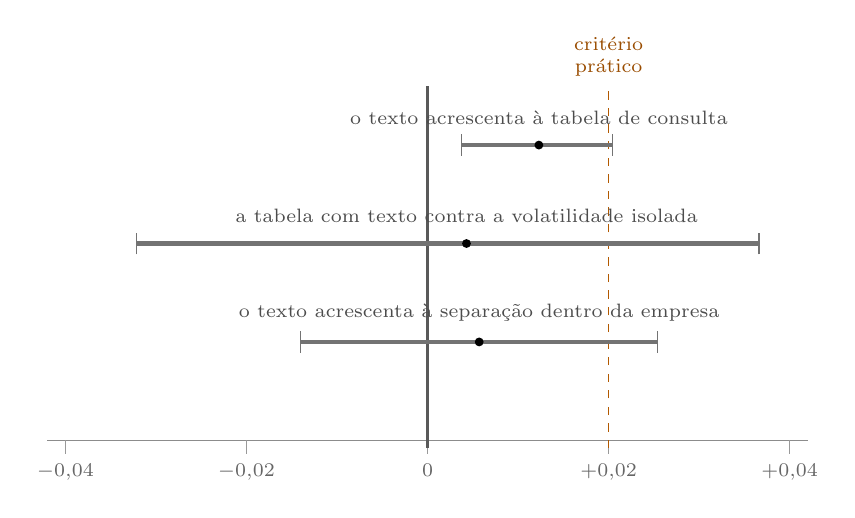
\begin{tikzpicture}[font=\small, x=115cm, y=1.25cm]
  \draw[black!45] (-0.042,0) -- (0.042,0);
  \foreach \xv/\xl in {-0.04/{$-0{,}04$}, -0.02/{$-0{,}02$}, 0/{$0$}, 0.02/{$+0{,}02$},
                       0.04/{$+0{,}04$}} {
    \draw[black!40] (\xv,0) -- (\xv,-0.14) node[below, font=\scriptsize, black!60] {\xl};
  }
  \draw[thick, black!65] (0,-0.08) -- (0,3.60);
  \draw[dashed, orange!70!black] (0.02,-0.08) -- (0.02,3.60)
    node[above, font=\scriptsize, text=orange!60!black, align=center] {critério\\ prático};

  \foreach \yv/\xa/\xm/\xb/\xrot in {
    3/0.0038/0.0123/0.0204/{o texto acrescenta à tabela de consulta},
    2/-0.0321/0.0043/0.0366/{a tabela com texto contra a volatilidade isolada},
    1/-0.0140/0.0057/0.0254/{o texto acrescenta à separação dentro da empresa}} {
    \draw[line width=1.6pt, black!55] (\xa,\yv) -- (\xb,\yv);
    \draw[black!55] (\xa,\yv-0.11) -- (\xa,\yv+0.11);
    \draw[black!55] (\xb,\yv-0.11) -- (\xb,\yv+0.11);
    \fill[black] (\xm,\yv) circle (1.6pt);
    \node[above=4pt, font=\scriptsize, black!70, align=center] at (\xm,\yv) {\xrot};
  }
\end{tikzpicture}
\caption[Os três acréscimos, com intervalo de confiança]{Diferenças de desempenho e respetivos
intervalos de confiança a noventa e cinco por cento, obtidos por reamostragem por grupos. As duas
primeiras linhas são diferenças de \gls{PRAUC} e a terceira é uma diferença de capacidade de
ordenação dentro de cada empresa. Apenas a primeira exclui zero, e fá-lo abaixo do critério prático
fixado antes da medição.}
\label{fig:av_acrescimo}
\end{figure}

O título acrescenta a essa base $+0{,}012$ de \gls{PRAUC}, com intervalo entre $+0{,}004$ e
$+0{,}020$, que exclui zero. É a primeira ocasião em que uma representação de texto apresenta um
acréscimo detetável nesta tarefa, e o valor situa-se abaixo do critério prático de $0{,}02$ fixado
antes dos resultados.

Três reservas delimitam o alcance deste acréscimo, e todas são medições. A primeira é que a soma não
supera a volatilidade isolada: o valor obtido é de $0{,}547$ contra $0{,}542$, e a diferença tem
intervalo entre $-0{,}032$ e $+0{,}037$, que contém zero. A segunda é que o acréscimo não chega ao produto. A precisão dentro do orçamento de cinco alertas
por dia é de $0{,}662$ com e sem o texto, sem uma casa decimal de diferença. O acréscimo existe na
ordenação do conjunto completo e desaparece quando apenas cinco notícias por dia são selecionadas.

A terceira é que o texto
continua a não separar notícias da mesma empresa. A capacidade de ordenação dentro de cada empresa
vale $0{,}500$ por construção para a tabela de consulta e sobe para $0{,}512$ quando se lhe soma o
título. Para o modelo implantado é de $0{,}502$, com intervalo entre $0{,}462$ e $0{,}542$, e sobe
para $0{,}508$ com o texto, num acréscimo de $+0{,}006$ cujo intervalo, entre $-0{,}014$ e
$+0{,}025$, contém zero. Nenhum dos dois se distingue do acaso. A informação que o texto traz distingue empresas e períodos, e não
notícias.

A resposta à \gls{QI}3 mantém-se negativa e torna-se mais precisa. Nenhum modelo com texto supera a
volatilidade, e o texto não é inútil: acrescenta ao que o modelo já conhece sobre a empresa, de forma
pequena e mensurável. O que impede esse acréscimo de alterar o sistema não é a ausência de
informação, mas a natureza da informação, que distingue empresas quando o produto necessita de
distinguir notícias. O trabalho seguinte requer um rótulo por notícia, e não apenas um modelo de
maior dimensão.

Uma reserva final aplica-se ao próprio método. Este é mais um modelo avaliado sobre o mesmo bloco de
teste, que já serviu várias comparações do capítulo, e quanto mais vezes um conjunto de teste é
observado, mais provável se torna encontrar nele uma diferença pequena. As duas defesas utilizadas,
que consistem em não afinar a configuração e em declarar o critério antes da medição, reduzem esse
risco sem o eliminarem. A formulação que subsiste é a mais fraca das possíveis: não é possível
rejeitar que o título acrescente informação, e o acréscimo, a existir, é inferior ao critério prático
fixado antes da medição. Trata-se de um limite superior de um efeito e não de uma descoberta.

\subsection{Limites da conclusão}

O resultado não estabelece que o texto de notícias seja inútil. Foi avaliada uma única representação,
constituída por títulos sem o corpo do artigo, sobre um único corpus. Com textos completos e maior
volume de dados a resposta poderia ser distinta, o que constitui trabalho futuro.

Existe ainda uma hipótese alternativa que estas medições não excluem. O rótulo desconta o movimento
do mercado assumindo sensibilidade unitária, pela incoerência declarada na
Secção~\ref{sec:met_triagem}. Numa ação de sensibilidade elevada, o resíduo da subtração retém
movimento do mercado, pelo que o erro do rótulo não é aleatório: é maior nas ações mais sensíveis ao
mercado, que são tipicamente também as mais voláteis. Ora a linha de base vencedora é exatamente a
volatilidade. Com o que está medido não é possível separar a hipótese de a volatilidade prever melhor
a materialidade da hipótese de a volatilidade prever melhor o erro introduzido pelo rótulo. A experiência que resolveria a questão consiste em reconstruir o alvo com sensibilidades estimadas
e encolhidas, como faz a Secção~\ref{sec:met_decomposicao}, e repetir as seis famílias. Não foi
realizada. O nível e a ordenação das métricas ficam condicionados ao rótulo utilizado.

\section{O que permanece mensurável na decomposição}
\label{sec:av_decomposicao}

A decomposição do movimento não dá origem a uma questão de investigação. Esta secção estabelece a
razão dessa ausência e o que, apesar dela, permanece falsificável na técnica.

A diferença face às três técnicas anteriores é a existência de um alvo externo. Para a deteção existe
um critério de movimento extremo, o que permite contar acertos e falhas; para a recuperação existe
uma noção verificável de relevância, de que decorre a precisão@$k$; para a triagem existe um rótulo
construído a partir de preços posteriores. Em todos estes casos a técnica pode revelar-se errada
contra um alvo que lhe é exterior.

Na decomposição esse alvo não existe. Nenhuma fonte de dados publica qual foi a parcela verdadeira do
mercado no movimento de uma ação num dado dia, uma vez que essa quantidade não é observável e apenas
existe relativamente a um modelo. Fixadas as sensibilidades, a repartição é uma identidade
contabilística e não uma previsão suscetível de sair certa ou errada. A construção de uma medida de
exatidão neste ponto produziria um valor sem referente.

A técnica não fica por avaliar, mas por avaliar dessa forma, o que obriga a determinar o que nela
permanece falsificável. São duas propriedades, e ambas se medem sobre as dezassete empresas do mapa
de setores, que é o conjunto percorrido pelo procedimento de avaliação e não a lista monitorizada em
produção. A Figura~\ref{fig:av_motor} apresenta as duas.

\begin{figure}[ht]
\centering
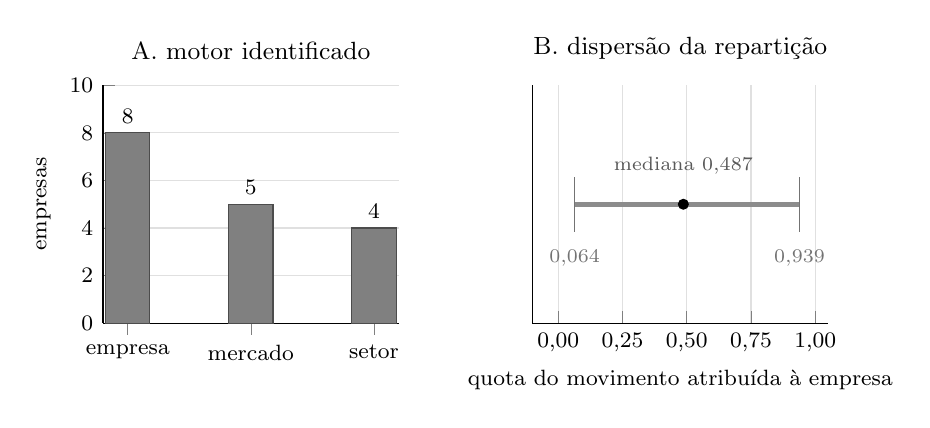
\begin{tikzpicture}
\begin{axis}[
  name=pa, width=0.44\textwidth, height=4.6cm, ybar, bar width=16pt,
  ymin=0, ymax=10, symbolic x coords={emp, merc, set}, xtick=data,
  xticklabels={empresa, mercado, setor}, ylabel={empresas},
  nodes near coords, point meta=explicit symbolic,
  every node near coord/.append style={font=\footnotesize},
  title={\small A. motor identificado},
  tick label style={font=\footnotesize}, label style={font=\footnotesize},
  ymajorgrids, grid style={black!12}, axis lines*=left,
]
\addplot[fill=black!50, draw=black!70] coordinates {(emp,8) [8] (merc,5) [5] (set,4) [4]};
\end{axis}
\begin{axis}[
  name=pb, at={(pa.right of origin)}, anchor=left of origin, xshift=1.7cm,
  width=0.44\textwidth, height=4.6cm,
  xmin=-0.10, xmax=1.05, ymin=0.4, ymax=1.6,
  ytick=\empty, xtick={0,0.25,0.5,0.75,1.0},
  xticklabels={{0,00},{0,25},{0,50},{0,75},{1,00}},
  xlabel={quota do movimento atribuída à empresa},
  title={\small B. dispersão da repartição},
  tick label style={font=\footnotesize}, label style={font=\footnotesize},
  xmajorgrids, grid style={black!12}, axis lines*=left,
]
\draw[line width=1.8pt, black!45] (axis cs:0.064,1) -- (axis cs:0.939,1);
\draw[black!55] (axis cs:0.064,0.86) -- (axis cs:0.064,1.14);
\draw[black!55] (axis cs:0.939,0.86) -- (axis cs:0.939,1.14);
\fill[black] (axis cs:0.487,1) circle (2pt);
\node[font=\scriptsize, black!65, anchor=south] at (axis cs:0.487,1.10) {mediana $0{,}487$};
\node[font=\scriptsize, black!55, anchor=north] at (axis cs:0.064,0.82) {$0{,}064$};
\node[font=\scriptsize, black!55, anchor=north] at (axis cs:0.939,0.82) {$0{,}939$};
\end{axis}
\end{tikzpicture}
\caption[A decomposição discrimina entre empresas no mesmo dia]{As dezassete empresas do mapa de
setores, decompostas no mesmo dia. Em A, a componente identificada como maior parcela do mesmo sinal
que o movimento observado. Em B, a dispersão da quota atribuída à empresa. A repartição produz
respostas distintas para empresas distintas no mesmo dia, que é a condição mínima para a sua
utilidade.}
\label{fig:av_motor}
\end{figure}

A primeira propriedade é a capacidade de discriminar. Uma decomposição que atribuísse a totalidade do
movimento à empresa em todos os dias seria inútil ainda que aritmeticamente correta. No dia medido, o
motor identificado foi a própria empresa em oito casos, o mercado em cinco e o setor em quatro, e a
quota do movimento atribuída à empresa apresentou mediana de $0{,}487$, com extremos em $0{,}064$ e
$0{,}939$.

A segunda propriedade é a qualidade da estimação das sensibilidades, e é a que pode efetivamente
estar errada. A medida apropriada é o coeficiente de determinação na janela de estimação, cuja
mediana foi de $0{,}460$. Não se trata do coeficiente do ajuste por mínimos quadrados, que, calculado
dentro da amostra e com termo constante, nunca poderia ser negativo, mas do coeficiente do modelo
efetivamente utilizado, com as sensibilidades já encolhidas e o termo constante recentrado. É esta a
medida adequada, por corresponder ao modelo cuja repartição é apresentada ao utilizador, e é por essa
razão que pode assumir valor negativo. Numa das dezassete empresas assumiu, o que significa que,
naquela janela, o mercado e o setor não explicavam a variação daquela ação melhor do que a sua própria
média, e que a repartição desse dia assenta num ajuste que não descreve os dados.

O resultado não estabelece que a repartição esteja correta pelo facto de as parcelas somarem. Elas
somam sempre, com diferença nula até à precisão da máquina, porque a parcela da empresa é definida
como resíduo, e uma repartição sem qualquer significado somaria igualmente. A soma exata constitui
uma verificação de implementação e não uma validação de método. O resultado também não estabelece que
o valor apresentado ao utilizador seja fiável em todos os dias, o que no caso de coeficiente negativo
não sucede, e é por essa razão que a limitação consta do Capítulo~\ref{cap:conclusoes}.

\section{O sistema em operação}
\label{sec:av_producao}

O quarto caso de estudo incide sobre o comportamento do sistema depois de implantado, sobre as
decisões que toma autonomamente. É a avaliação menos comum das três descritas na
Secção~\ref{sec:met_metodologia}, e a que produz o diagnóstico que alterou o sistema.

\subsection{O que a porta de decisão estava a separar}

A porta implantada era um limiar fixo sobre a probabilidade calibrada, que deixava passar as
candidatas acima de $0{,}50$. A pergunta com significado é a de saber se esse limiar separava títulos
ou separava empresas, e a medição foi realizada sobre as $4\,366$ decisões efetivamente tomadas em
produção. A Figura~\ref{fig:av_porta} apresenta o resultado.

\begin{figure}[ht]
\centering
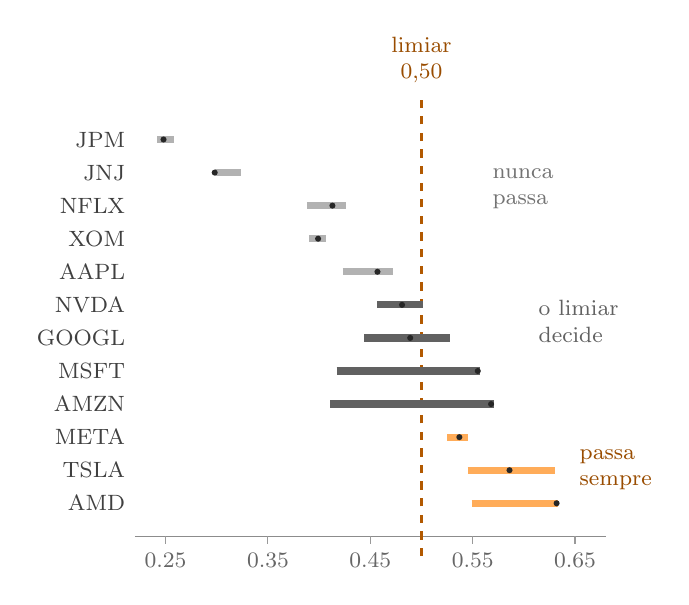
\begin{tikzpicture}[font=\footnotesize, x=13cm, y=0.42cm]
  \draw[black!45] (0.22,0) -- (0.68,0);
  \foreach \xv in {0.25,0.35,0.45,0.55,0.65}
    \draw[black!40] (\xv,0) -- (\xv,-0.22) node[below, black!60] {\xv};
  \draw[dashed, thick, orange!70!black] (0.50,-0.6) -- (0.50,13.4)
    node[above, align=center, text=orange!60!black] {limiar\\ $0{,}50$};
  \foreach \xn/\xtk/\xa/\xm/\xb/\xcor in {
    12/JPM/0.242/0.248/0.258/black!30, 11/JNJ/0.298/0.298/0.324/black!30,
    10/NFLX/0.388/0.413/0.426/black!30, 9/XOM/0.390/0.399/0.407/black!30,
    8/AAPL/0.423/0.457/0.472/black!30, 7/NVDA/0.457/0.481/0.501/black!62,
    6/GOOGL/0.444/0.489/0.528/black!62, 5/MSFT/0.417/0.555/0.557/black!62,
    4/AMZN/0.411/0.568/0.571/black!62, 3/META/0.525/0.537/0.545/orange!65,
    2/TSLA/0.545/0.586/0.630/orange!65, 1/AMD/0.549/0.632/0.633/orange!65}
  {
    \node[left, black!75] at (0.22,\xn) {\xtk};
    \draw[line width=2.6pt, color=\xcor] (\xa,\xn) -- (\xb,\xn);
    \fill[black!85] (\xm,\xn) circle (1.1pt);
  }
  \node[right, align=left, text=orange!60!black] at (0.645,2) {passa\\ sempre};
  \node[right, align=left, black!55] at (0.56,10.5) {nunca\\ passa};
  \node[right, align=left, black!62] at (0.605,6.5) {o limiar\\ decide};
\end{tikzpicture}
\caption[O que a porta de decisão separava]{Intervalo de todas as pontuações atribuídas pelo modelo a
cada empresa em produção, com a mediana assinalada. As barras claras nunca alcançam o limiar, as
escuras atravessam-no e as alaranjadas situam-se sempre acima. Oito das doze empresas encontram-se
inteiramente de um dos lados, o que significa que para essas a decisão estava tomada antes de o
título ser lido.}
\label{fig:av_porta}
\end{figure}

Os valores confirmam a leitura da figura. Sobre as $36\,925$ decisões registadas, a amplitude média
das pontuações dentro de cada empresa é de $0{,}072$, ao passo que a amplitude entre as medianas das
empresas é de $0{,}392$, isto é, $5{,}4$ vezes superior. Duas empresas situavam-se sempre acima do
limiar e cinco nunca o alcançavam, pelo que apenas em cinco das doze o limiar chegava a decidir. Em $48\%$ dos títulos distintos o resultado estava determinado pela empresa antes de o título ser
lido. Contada por decisão registada, a fração sobe para $60\%$. Cita-se a primeira: a repontuação
dos mesmos títulos a cada ciclo de sessenta segundos inflaciona a segunda, e de forma desigual
entre empresas.

Numa janela anterior e mais curta, de $4\,366$ decisões, os mesmos
indicadores valiam $0{,}064$, $0{,}385$ e $6{,}1$ vezes, com três empresas sempre acima e quatro em
que o limiar decidia. A conclusão estrutural não depende da janela. Em nenhuma das avaliações
registadas a Apple alcançou o limiar, com um máximo observado de $0{,}472$, ao passo que a AMD o
ultrapassou em todas.

As duas contagens medem quantidades distintas e ambas são reportadas. O sistema repontua os mesmos
títulos a cada ciclo de sessenta segundos, e a duplicação é maior nas empresas com menos notícias,
que são as que nunca ultrapassam o limiar, pelo que contar decisões desloca a fração para cima.
Contada uma vez por título distinto, sobre uma janela mais ampla de $36\,925$ decisões, a fração é de
$48\%$. A conclusão estrutural não depende da contagem escolhida: continuam a existir empresas
inteiramente de um dos lados do limiar, e a amplitude entre empresas continua a ser várias vezes a
amplitude dentro de cada uma.

O defeito tem a mesma forma que o identificado na Secção~\ref{sec:av_qi1}, uma camada acima. Naquele
caso, um limiar fixo sobre o retorno mede a volatilidade da empresa em vez da raridade do dia; neste,
um limiar fixo sobre uma pontuação quase constante por empresa ordena empresas em vez de notícias.

Nenhum dos testes automáticos existentes o cobria. O modelo foi avaliado sobre a distribuição do
conjunto de treino e implantado atrás de dois filtros que a alteram, e cada componente cumpria o seu
contrato. O teste que o teria apanhado é o que este trabalho passou a executar: comparar a amplitude
das pontuações dentro de cada empresa com a amplitude entre empresas. O
que estava errado era uma suposição sobre a ligação entre eles, não enunciada em nenhum ponto.
Corresponde à classe de custo que \textcite{sculley2015debt} arrumam sob dependências de dados e
emaranhamento entre componentes, com o sintoma que os autores descrevem: o sistema continua a
produzir valores de aparência normal.

Existe uma segunda causa possível, que os registos não permitem separar da primeira. Uma das nove entradas é o retorno do próprio dia. No treino corresponde ao movimento completo do
dia da notícia. Em produção é calculado sobre a última barra diária disponível, que durante a
sessão é o fecho da véspera ou uma barra incompleta. As duas causas produzem o mesmo sintoma, e o registo
guarda a probabilidade e o resultado mas não o valor das entradas no momento da pontuação. A sua
separação exigiria registar essas entradas e voltar a observar durante semanas.

A correção aparente consistiria em substituir o limiar fixo por um limiar relativo a cada empresa. A simulação dessa alternativa sobre as mesmas decisões resolve metade do problema, uma vez que as
doze empresas passam a estar representadas, e introduz outro. Nas empresas cuja pontuação quase
não varia, o percentil recai sobre a constante e quase todas as decisões empatam acima dele; uma
delas passa a gerar $874$ alertas. O limiar relativo deixa de escolher por materialidade e passa a
escolher por desempate, que é precisamente o artefacto documentado na Secção~\ref{sec:av_qi3}. Dentro
de uma empresa a pontuação do modelo quase não varia com o título, e nenhuma regra de decisão
aplicada a essa pontuação a pode tornar sensível à notícia, porque a informação que distinguiria um
título do seguinte não está presente.

Em consequência, o modelo deixou de constituir porta e passou a constituir critério de ordenação, que
é a utilização que a medição sustenta, e o controlo de volume passou para um orçamento diário de
cinco alertas. Esta alteração aproxima duas políticas que divergiam: a dissertação avaliava uma
política de orçamento e o sistema implantava uma política de limiar, pelo que o valor reportado
descrevia um sistema distinto do que estava em funcionamento. As duas políticas passaram a pertencer
à mesma família sem se tornarem idênticas.

A métrica avaliada ordena todas as candidatas do bloco de
teste e apenas depois preenche cinco lugares em cada dia, o que exige conhecer o dia completo antes
de decidir e constitui por isso uma política diferida. O sistema implantado decide em linha, de
sessenta em sessenta segundos, e gasta o primeiro lugar na primeira notícia que atravesse as portas,
porque no momento da decisão a notícia da tarde ainda não existe. A precisão dentro do orçamento
reportada neste capítulo é, por conseguinte, um limite superior do que a política implantada obtém.

\subsection{O desempenho do modelo sobre as decisões que tomou}

O sistema regista todas as decisões de triagem e, decorridos os dias necessários para o preço
responder, confronta-as com o resultado efetivo. Duas medições resultam desse registo: a fração de
casos que se revelaram materiais de cada lado da porta, e a capacidade de ordenação do modelo,
medida pela \gls{ROCAUC}. A Figura~\ref{fig:av_posvalidacao} apresenta ambas, sobre $825$ decisões
já maturadas.

\begin{figure}[ht]
\centering
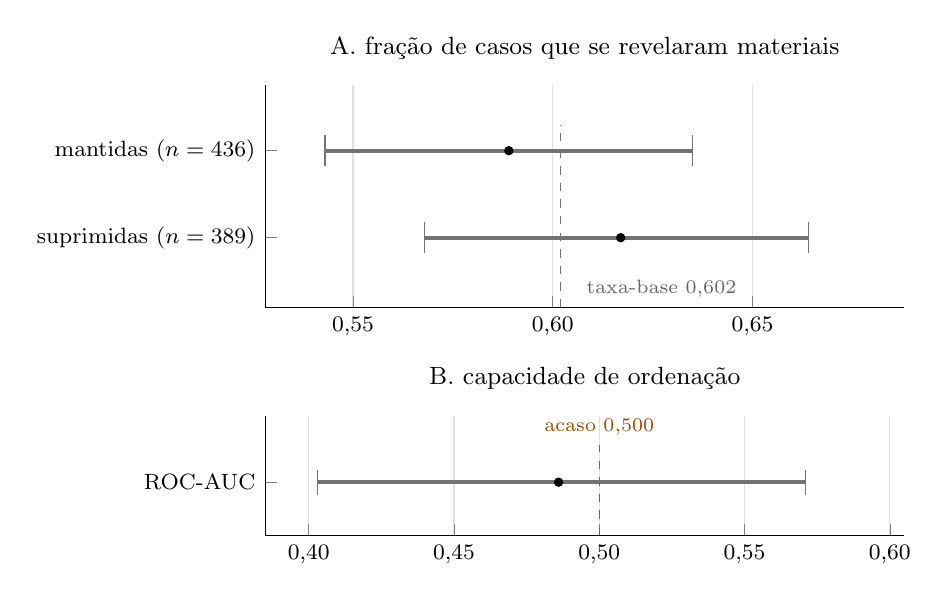
\begin{tikzpicture}
\begin{axis}[
  name=pa, width=0.80\textwidth, height=4.4cm,
  xmin=0.528, xmax=0.688, ymin=0.20, ymax=2.75,
  ytick={1,2}, yticklabels={{suprimidas ($n = 389$)}, {mantidas ($n = 436$)}},
  xtick={0.55,0.60,0.65}, xticklabels={{0,55},{0,60},{0,65}},
  title={\small A. fração de casos que se revelaram materiais},
  tick label style={font=\footnotesize}, label style={font=\footnotesize},
  xmajorgrids, grid style={black!12}, axis lines*=left,
]
\addplot[draw=none, forget plot] coordinates {(0.60,1.5)};
\draw[dashed, black!55] (axis cs:0.602,0.20) -- (axis cs:0.602,2.30);
\node[font=\scriptsize, black!60, anchor=west] at (axis cs:0.606,0.42) {taxa-base $0{,}602$};
\draw[line width=1.4pt, black!55] (axis cs:0.543,2) -- (axis cs:0.635,2);
\draw[black!55] (axis cs:0.543,1.82) -- (axis cs:0.543,2.18);
\draw[black!55] (axis cs:0.635,1.82) -- (axis cs:0.635,2.18);
\fill[black] (axis cs:0.589,2) circle (1.7pt);
\draw[line width=1.4pt, black!55] (axis cs:0.568,1) -- (axis cs:0.664,1);
\draw[black!55] (axis cs:0.568,0.82) -- (axis cs:0.568,1.18);
\draw[black!55] (axis cs:0.664,0.82) -- (axis cs:0.664,1.18);
\fill[black] (axis cs:0.617,1) circle (1.7pt);
\end{axis}
\begin{axis}[
  name=pb, at={(pa.below south west)}, anchor=north west, yshift=-9mm,
  width=0.80\textwidth, height=3.1cm,
  xmin=0.385, xmax=0.605, ymin=0.4, ymax=1.75,
  ytick={1}, yticklabels={ROC-AUC},
  xtick={0.40,0.45,0.50,0.55,0.60},
  xticklabels={{0,40},{0,45},{0,50},{0,55},{0,60}},
  title={\small B. capacidade de ordenação},
  tick label style={font=\footnotesize}, label style={font=\footnotesize},
  xmajorgrids, grid style={black!12}, axis lines*=left,
]
\addplot[draw=none, forget plot] coordinates {(0.50,1)};
\draw[dashed, orange!70!black] (axis cs:0.50,0.4) -- (axis cs:0.50,1.42);
\node[font=\scriptsize, text=orange!60!black, anchor=south] at (axis cs:0.50,1.42)
  {acaso $0{,}500$};
\draw[line width=1.4pt, black!55] (axis cs:0.403,1) -- (axis cs:0.571,1);
\draw[black!55] (axis cs:0.403,0.86) -- (axis cs:0.403,1.14);
\draw[black!55] (axis cs:0.571,0.86) -- (axis cs:0.571,1.14);
\fill[black] (axis cs:0.486,1) circle (1.7pt);
\end{axis}
\end{tikzpicture}
\caption[O modelo sobre as decisões que tomou em produção]{Em A, a fração de casos que se revelaram
materiais entre as decisões que o modelo deixou passar e entre as que travou, com intervalos de
confiança a noventa e cinco por cento e a taxa-base do conjunto. As suprimidas apresentam fração
superior às mantidas, mas os dois intervalos sobrepõem-se em quase toda a extensão e não as
separam. Em B, a capacidade de ordenação medida sobre as $239$ unidades independentes, com o
intervalo a conter confortavelmente o valor de acaso.}
\label{fig:av_posvalidacao}
\end{figure}

Sobre a população que efetivamente observa, esta amostra não distingue o modelo do acaso em nenhuma
das duas medidas. As notícias que deixou passar revelaram-se materiais em $58{,}9\%$ dos casos,
contra $61{,}7\%$ das que travou, sobre uma taxa-base de $60{,}2\%$; os intervalos das duas frações
sobrepõem-se, pelo que a ordenação aparente não é estabelecida. O que fica medido é a ausência de
benefício detetável com esta dimensão de amostra, e não a ausência de benefício.

Estes valores exigem uma reserva de precisão considerável: as $825$ decisões
não constituem $825$ observações independentes, dado que o rótulo é atribuído por par formado pela
empresa e pelo dia, e as linhas repartem-se por apenas $239$ pares distintos. Medida sobre essas
unidades, a capacidade de ordenação situa-se em $0{,}486$ com intervalo de confiança entre $0{,}403$
e $0{,}571$, num intervalo em que o acaso vale exatamente $0{,}500$. A leitura correta não é a de que
o modelo seja pior do que a ausência de modelo, mas a de que esta amostra não o distingue do acaso.

A medição foi repetida quando o registo dispunha de $825$ decisões maturadas contra as $530$ da
primeira leitura, e quase nada se alterou: a diferença entre mantidas e suprimidas estreitou-se, a
capacidade de ordenação passou de $0{,}494$ para $0{,}486$ e o intervalo encolheu. Com metade mais
evidência, o veredicto mantém-se e torna-se mais firme.

A explicação mais provável não é a de que o modelo esteja avariado, mas a de que esteja em excesso.
Quando é invocado, as notícias já atravessaram o filtro de relevância e o filtro de frescura, e esses
filtros elementares removeram grande parte daquilo que o modelo foi treinado para remover, restando
pouco para separar. Um modelo avaliado isoladamente e implantado atrás de filtros nunca foi avaliado
na distribuição que efetivamente observa, e esta é a constatação com maior capacidade de
transferência do trabalho.

Três das doze empresas monitorizadas, a AMD, a Netflix e a Meta, não figuram no corpus de treino, e
uma quarta, a Microsoft, figura apenas no bloco de teste. O modelo pontua-as na mesma, porque o que
recebe são valores numéricos e não a identidade da empresa, mas fá-lo sobre uma combinação de
entradas que não observou. Duas das ausentes, a AMD e a Meta, estão entre as que se situam sempre
acima do limiar, pelo que a determinação por empresa descrita acima se concentra precisamente em
nomes que o modelo nunca observou. Constitui um segundo sentido, mais literal, em que o modelo
implantado opera fora da distribuição em que foi avaliado, e as decisões dessas empresas entram
nas $825$ acima como quaisquer outras.

\subsection{Deriva das distribuições}

Uma segunda razão, independente da anterior, pode fazer com que um modelo implantado deixe de servir:
os dados alteram-se. O modelo foi treinado sobre o período de 2018 a 2023 e opera em 2026. A medida
utilizada é o \gls{PSI}, que confronta aqui a distribuição de cada entrada no bloco de treino,
compreendido entre 2018 e 2022, com a do bloco de teste, de 2023. Não é, portanto, a distância entre
o treino e o presente, que a subsecção seguinte discute em separado: é a deriva interna ao próprio
protocolo. As bandas são as convencionadas em risco de crédito, segundo as quais valores
abaixo de $0{,}10$
indicam estabilidade, valores entre $0{,}10$ e $0{,}25$ deslocamento moderado e valores acima de
$0{,}25$ deslocamento significativo. A Figura~\ref{fig:av_deriva} apresenta o resultado.

\begin{figure}[ht]
\centering
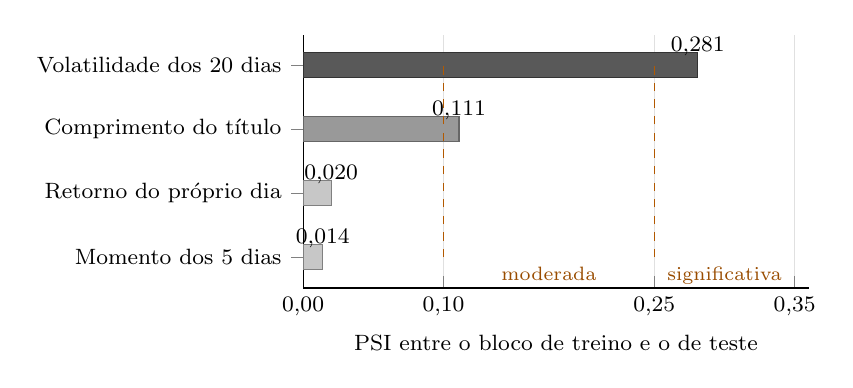
\begin{tikzpicture}
\begin{axis}[
  xbar, width=0.66\textwidth, height=4.8cm, bar width=9pt,
  xmin=0, xmax=0.36, enlarge y limits=0.16,
  symbolic y coords={mom, ret, comp, vol}, ytick={mom, ret, comp, vol},
  yticklabels={Momento dos 5 dias, Retorno do próprio dia, Comprimento do título,
               Volatilidade dos 20 dias},
  nodes near coords, nodes near coords align={horizontal}, point meta=explicit symbolic,
  every node near coord/.append style={font=\footnotesize},
  xlabel={\gls{PSI} entre o bloco de treino e o de teste},
  xtick={0,0.10,0.25,0.35}, xticklabels={{0,00},{0,10},{0,25},{0,35}},
  tick label style={font=\footnotesize}, label style={font=\footnotesize},
  xmajorgrids, grid style={black!12}, axis lines*=left,
]
\addplot[bar shift=0pt, fill=black!22, draw=black!50] coordinates {(0.014,mom) [0,014] (0.020,ret) [0,020]};
\addplot[bar shift=0pt, fill=black!40, draw=black!60] coordinates {(0.111,comp) [0,111]};
\addplot[bar shift=0pt, fill=black!65, draw=black!80] coordinates {(0.281,vol) [0,281]};
\draw[dashed, orange!70!black] (axis cs:0.10,mom) -- (axis cs:0.10,vol);
\draw[dashed, orange!70!black] (axis cs:0.25,mom) -- (axis cs:0.25,vol);
\node[font=\scriptsize, text=orange!60!black, anchor=north] at (axis cs:0.175,mom) {moderada};
\node[font=\scriptsize, text=orange!60!black, anchor=north] at (axis cs:0.30,mom)
  {significativa};
\end{axis}
\end{tikzpicture}
\caption[Deslocamento das distribuições de entrada]{Índice de estabilidade populacional de cada
entrada entre o bloco de treino, de 2018 a 2022, e o bloco de teste, de 2023, com as bandas
convencionadas assinaladas. A entrada de que o modelo mais depende é a que mais se deslocou. A
prevalência do rótulo passa de $0{,}3854$ para $0{,}3781$ entre as duas pontas, mas não é estável
pelo meio: no bloco de validação, temporalmente entre ambas, chega a $0{,}4704$.}
\label{fig:av_deriva}
\end{figure}

O resultado tem duas metades. A entrada que mais se deslocou é a volatilidade dos vinte dias
anteriores, situada na banda significativa, ao passo que as restantes permanecem estáveis ou
moderadas. O rótulo desloca-se pouco entre as pontas, com a prevalência de positivos a passar de
$0{,}3854$ para $0{,}3781$, mas não é estável: o bloco de validação, temporalmente entre os dois,
chega a $0{,}4704$. A prevalência oscila com o regime de volatilidade em vez de derivar numa
direção, o que é coerente com a volatilidade ser a entrada que mais se desloca.

A leitura correta desta medição é a de que a deriva não é externa aos valores deste capítulo: é a
que o próprio protocolo atravessa, uma vez que treina em 2018--2022 e avalia em 2023. A \gls{PRAUC}
reportada é já uma medida sob esta deriva, e a combinação é desfavorável porque a entrada de que o
modelo mais depende é precisamente a que mais se deslocou.

O que esta medição não estabelece é a distância entre o treino e 2026, que é o período em que o
sistema opera. Um instantâneo sobre cotações atuais aponta na mesma direção, com a volatilidade a ser de novo a
entrada que mais se desloca. Assenta, porém, em janelas deslizantes consecutivas que partilham a
quase totalidade das observações, o que inflaciona o índice e torna a sua magnitude não comparável
com a da figura. Fica registado como não medido, em vez de estimado por analogia. A
deriva é, em qualquer dos casos, medida e não corrigida, e a Secção~\ref{sec:con_futuro} enuncia o
que seria necessário para a corrigir.

\subsection{O sistema completo contra as alternativas existentes}

As secções anteriores comparam componente a componente. Falta a comparação ao nível do sistema:
dadas as notícias de um dia, a política escolhe as cinco a apresentar melhor do que uma regra
disponível sem custo. A Figura~\ref{fig:av_pontaaponta} responde. Todas as políticas escolhem cinco
por dia, sobre o mesmo bloco de teste e com o mesmo rótulo, e o desempate é aleatório e explícito em
todas.

\begin{figure}[ht]
\centering
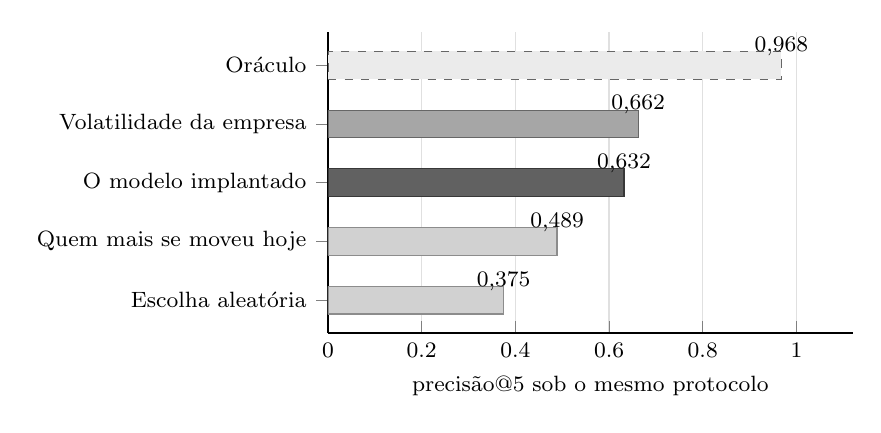
\begin{tikzpicture}
\begin{axis}[
  xbar, width=0.68\textwidth, height=5.4cm, bar width=10pt,
  xmin=0, xmax=1.12, enlarge y limits=0.14,
  symbolic y coords={acaso, mexeu, modelo, volat, oraculo},
  ytick={acaso, mexeu, modelo, volat, oraculo},
  yticklabels={Escolha aleatória, Quem mais se moveu hoje, O modelo implantado,
               Volatilidade da empresa, Oráculo},
  nodes near coords, nodes near coords align={horizontal}, point meta=explicit symbolic,
  every node near coord/.append style={font=\footnotesize},
  xlabel={precisão@5 sob o mesmo protocolo},
  tick label style={font=\footnotesize}, label style={font=\footnotesize},
  xmajorgrids, grid style={black!12}, axis lines*=left,
]
\addplot[bar shift=0pt, fill=black!18, draw=black!45] coordinates {(0.375,acaso) [0,375] (0.489,mexeu) [0,489]};
\addplot[bar shift=0pt, fill=black!62, draw=black!78] coordinates {(0.632,modelo) [0,632]};
\addplot[bar shift=0pt, fill=black!35, draw=black!60] coordinates {(0.662,volat) [0,662]};
\addplot[bar shift=0pt, fill=black!8, draw=black!60, dashed] coordinates {(0.968,oraculo) [0,968]};
\end{axis}
\end{tikzpicture}
\caption[O sistema contra as alternativas já disponíveis]{Cinco políticas de seleção sobre o mesmo
bloco de teste. A primeira e a última não são políticas utilizáveis: uma é o valor de referência e a
outra é o máximo teórico, obtido com conhecimento das respostas. Todas escolhem conhecendo o dia
completo, pelo que cada valor é um limite superior do que a mesma regra obteria decidindo ao minuto.}
\label{fig:av_pontaaponta}
\end{figure}

Três leituras resultam da figura. A primeira é que o sistema supera a alternativa realista: apresentar
notícias das empresas com maior movimento do dia é o que qualquer aplicação de bolsa já faz sem
custo, e obtém $0{,}489$, contra $0{,}632$ do sistema, um ganho de $0{,}143$ sob o mesmo protocolo.
Este valor mede a capacidade de ordenar o rótulo aproximado no bloco histórico, e não a utilidade
percebida por uma pessoa nem o valor causal dos alertas em funcionamento.

A segunda é que o sistema continua a não superar a volatilidade. Treze constantes calculadas
exclusivamente sobre o bloco de treino obtêm $0{,}662$, o que é coerente com a ablação da
Secção~\ref{sec:av_ablacao}: o modelo é, na prática, uma tabela por empresa, e a volatilidade é outra
tabela por empresa, mais simples, sendo esta a que dispensa treino.

A terceira, e mais útil, é a localização da limitação pelo máximo teórico. O melhor resultado
possível, escolhendo com conhecimento das respostas, seria de $0{,}968$, o que significa que em quase
todos os dias existem efetivamente cinco notícias materiais no conjunto disponível. O sistema não
está limitado por escassez de matéria-prima, mas pela incapacidade de identificar quais são. A margem
entre $0{,}632$ e $0{,}968$ é de $0{,}336$ e reside quase integralmente na separação de notícias
dentro de cada empresa, que é precisamente o que o modelo implantado não consegue realizar. É a mesma
conclusão obtida por um terceiro caminho independente.

Todas as políticas desta comparação escolhem de entre o que a fonte entregou, o que deixa de fora a
pergunta anterior a todas, relativa aos dias em que nada foi entregue. Sobre um ano de notícias
captadas, existia pelo menos uma notícia relevante em $88{,}5\%$ dos dias que o detetor considerou
invulgares, num total de $417$, e em $47$ dos $52$ dias mais extremos, dimensão que não permite
distinguir as duas frações. Nos restantes, nenhuma alteração ao sistema produz
efeito, uma vez que uma notícia não associada à empresa pela fonte gratuita não chega a entrar no
percurso. A cobertura é ainda muito desigual, com a empresa pior coberta a situar-se nos $50\%$. Este
valor é um limite superior, e a distinção determina o que ele vale: estabelece que existia uma
notícia, e não que tenha chegado a notícia correta. A Secção~\ref{sec:con_limitacoes} retoma-o como
limitação.

Uma linha de base não foi medida, e a razão fica registada. A alternativa mais natural consistiria em
apresentar as primeiras cinco notícias a chegar. Não é mensurável neste protocolo, uma vez que o
conjunto de dados histórico não conserva a hora de publicação e está ordenado por data e por empresa,
pelo que utilizar a ordem do ficheiro mediria a ordem alfabética das empresas. Seria o mesmo
artefacto documentado na Secção~\ref{sec:av_qi3}, desta vez introduzido deliberadamente. Uma linha de
base errada é pior do que uma linha de base em falta.

\section{Síntese dos resultados}
\label{sec:av_sintese}

Esta secção reúne as comparações realizadas ao longo do trabalho, incluindo aquelas em que o sistema
mantém a opção que a medição não favorece.

Duas das três respostas são afirmativas e uma é negativa. A resposta negativa é a que exigiu maior
esforço de verificação, e é também a que estabelece que a avaliação foi construída de modo a poder
produzir uma resposta negativa. A Tabela~\ref{tab:av_alternativas} apresenta cada escolha técnica ao
lado da alternativa medida contra ela.

\begin{table}[!htbp]
\caption[Cada escolha, contra a alternativa que não ficou]{As decisões técnicas do trabalho, cada uma
com a alternativa medida contra ela. Três linhas registam que a opção implantada não obteve o melhor
resultado, e a razão da sua manutenção consta da coluna respetiva. As três últimas linhas não
apresentam valores por corresponderem a restrições fixadas antes de qualquer medição.}
\label{tab:av_alternativas}
\centering
\scriptsize
\begin{tabular}{L{0.19\textwidth} L{0.30\textwidth} L{0.39\textwidth}}
\toprule
\tabhead{Opção implantada} & \tabhead{Alternativa medida} & \tabhead{Leitura} \\
\midrule
\emph{z}-score deslizante & Limiar fixo de três por cento: amplitude $0{,}344$ contra $0{,}015$ &
Um limiar fixo mede a volatilidade da empresa e não a raridade do dia. \\
\addlinespace
\emph{z}-score deslizante & \emph{Isolation Forest} com $F_1$ de $0{,}269$ e \emph{Local Outlier
Factor} com $0{,}280$, contra $0{,}530$ & Os detetores aprendidos assinalam quase tudo e acertam
pouco. \\
\addlinespace
Janela de vinte dias & Não obteve o melhor resultado: dez dias produzem $F_1$ de $0{,}385$, vinte
dias $0{,}516$ e sessenta dias $0{,}678$ & A medição favorece a janela mais longa. Mantida por
responsividade, com a reserva de circularidade do rótulo declarada. \\
\addlinespace
Desvio-padrão de pesos iguais & Não obteve o melhor resultado: o decaimento exponencial produz $F_1$
de $0{,}664$ contra $0{,}516$ & Mantido por ser explicável a um leitor não especializado, e
registado como escolha e não como resultado. \\
\addlinespace
Embeddings de frase & Sobreposição de palavras: precisão@5 de $0{,}346$ contra $0{,}514$ &
Vocabulário comum não implica assunto comum, e assunto comum não exige vocabulário comum. \\
\addlinespace
MiniLM em vez de MPNet & Não obteve o melhor resultado: o MPNet produz $0{,}538$ contra $0{,}514$; um
codificador de domínio financeiro produz $0{,}420$ & O modelo mais pesado é melhor e foi substituído
por custo. O codificador de domínio obteve o pior resultado de todos, por medição e não por
suposição. \\
\addlinespace
Regressão logística & Árvores com reforço do gradiente: \gls{PRAUC} de $0{,}469$ contra $0{,}538$ &
O modelo mais expressivo não obteve melhor resultado, e o modelo simples é explicável. \\
\addlinespace
Calibração de Platt & Regressão isotónica, comparada sobre a mesma validação & A calibração de Platt
iguala ou supera no índice de Brier em todas as famílias avaliadas. \\
\addlinespace
Semelhança do cosseno & Distância euclidiana & Com vetores normalizados as duas produzem a mesma
ordenação, e a primeira dispõe de leitura mais direta. \\
\addlinespace
Dois gatilhos, notícia e preço & Fusão com o volume e a intensidade de notícia, na linha dos painéis
que combinam sinais de origens distintas \autocite{worldmonitor2026}: perde em dois dos três
orçamentos, com $-0{,}050$ e $-0{,}032$, e ganha no terceiro por $+0{,}004$ & Um ganho que depende do
orçamento escolhido, e uma ordem de grandeza menor do que as perdas, não sustenta a adoção. O volume
continua a ser calculado e apresentado como contexto, sem originar alertas. \\
\midrule
Apenas fontes gratuitas & --- & Restrição fundadora: define o público que o sistema pode servir. \\
Ausência de previsão de preços & --- & Restrição de desenho: é o que torna verificável tudo o
restante. \\
Mercado dos Estados Unidos & --- & Restrição de âmbito: é onde as fontes gratuitas apresentam
cobertura. \\
\bottomrule
\end{tabular}
\end{table}

Três linhas da tabela merecem desenvolvimento. A primeira respeita ao codificador de domínio
financeiro, cuja derrota tem explicação no objetivo de treino e não no conhecimento do domínio,
conforme a Secção~\ref{sec:av_qi2} estabelece. A segunda respeita à janela de vinte dias, que é a
opção mais difícil de justificar, uma vez que a única medição existente sobre este ponto não a
sustenta e a justificação de responsividade não é quantitativa. A terceira respeita ao estimador de
volatilidade, mantido por explicabilidade contra uma alternativa medida como superior.

As três últimas linhas não apresentam valores deliberadamente. São restrições e não resultados, tendo
sido fixadas antes de qualquer medição, e a sua apresentação sob a forma de comparação atribuir-lhes-ia
uma autoridade que não possuem.

O capítulo documenta três ocasiões em que uma técnica mais simples superou uma técnica mais
sofisticada em condições equivalentes, e duas ocasiões em que a técnica mais sofisticada obteve
melhor resultado e o sistema manteve a mais simples por explicabilidade. A distinção entre estes dois
casos é a distinção entre resultado e escolha, e o Capítulo~\ref{cap:conclusoes} retoma-a ao
estabelecer o que este trabalho demonstra e o que apenas decide.
